\documentclass[]{styles/svproc}  % Comment this line out

%\IEEEoverridecommandlockouts                              % This command is only
                                                          % needed if you want to
                                                          % use the \thanks command
%\overrideIEEEmargins

\usepackage{amsmath}    % need for subequations
\usepackage{amssymb}
\usepackage{graphicx}   % need for figures
\usepackage{color}      % use if color is used in text
\usepackage{subcaption}
\usepackage{algorithm}
\usepackage{algpseudocode}
\usepackage{url}
\usepackage{tikz}
\usepackage[outdir=./figures/]{epstopdf}
\def\UrlFont{\rmfamily}


% bounce transition graph
% visibility event graph
% bounce visibility diagram/graph

% synthesis of paths with high-level dynamical properties from simple
% compliant environmental interactions

% skeptical questions:

% - what if the robot starts very near to a boundary of equivalence classes?

% Using Visibility Equivalence Classes for High-Level Dynamical Path Synthesis

% Minimal (Complexity | Attention) Path Synthesis with Dynamical Specifications

%\title{Path Synthesis from Dynamical Specifications \\ for Blind Mobile Robots in Polygons}

%
%
%
%%%% list of authors for the TOC (use if author list has to be modified)
%\tocauthor{Ivar Ekeland, Roger Temam, Jeffrey Dean, David Grove,
%Craig Chambers, Kim B. Bruce, and Elisa Bertino}
%

\begin{document}
\mainmatter              % start of a contribution


% A Toolbox for
\title{A Visibility-Based Approach to Computing Nondeterministic Bouncing
Strategies}

\titlerunning{Nondeterministic Bouncing Strategies}  % abbreviated title (for running head)
%                                     also used for the TOC unless
%                                     \toctitle is used
\author{Alexandra Q. Nilles\inst{1} \and Yingying Ren\inst{1} \and Israel
Becerra\inst{1} \and Steven M. LaValle\inst{1}% <-this % stops a space
}
\authorrunning{A. Nilles, Y. Ren, I. Becerra, S. M. LaValle} % abbreviated author list (for running head)
%\thanks{This work was partially supported by National Science Foundation (award numbers ).}
%\institute{Princeton University, Princeton NJ 08544, USA,\\
%\email{I.Ekeland@princeton.edu},\\ WWW home page:
%\texttt{http://users/\homedir iekeland/web/welcome.html}
%\and
%Universit\'{e} de Paris-Sud,
%Laboratoire d'Analyse Num\'{e}rique, B\^{a}timent 425,\\
%F-91405 Orsay Cedex, France}

%\institute{University of Illinois at Urbana-Champaign}

\maketitle

%%%%%%%%%%%%%%%%%%%%%%%%%%%%%%%%%%%%%%%%%%%%%%%%%%%%%%%%%%%%%%%%%%%%%%%%%%%%%%%%
\begin{abstract}
Inspired by motion patterns of commercially available mobile robots, we investigate the power of robots that 
move forward in straight lines
until colliding with an environment boundary, at which point they can rotate in
place and move forward again; we visualize this as the robot ``bouncing" off
boundaries. Different boundary interaction laws can be
defined for such robots, such as ones which orient the robot relative to its
heading prior to collision, or relative to the normal vector of the environment
boundary. We introduce a data structure, generated from a polygonal environment
 definition and constraints on the robot's bouncing strategy, which can be
queried to determine the feasibility of path-based tasks such as navigation,
patrolling, coverage, and localization. If the task is feasible, this
approach then synthesizes a controller and calculates the maximum allowable 
uncertainty in the robot's actuation, providing design constraints for different 
environments and tasks.
\end{abstract}


\section{Introduction}

Mobile robots have rolled smoothly into our everyday lives, and can now be
spotted vacuuming our floors, cleaning our pools, mowing our grass, and moving
goods in our warehouses. These tasks require certain properties of
the robot's path through space: for example, a mowing or
vacuuming robot should cover the whole space while not visiting 
any particular area more frequently than others. A robot that is monitoring a space 
(such as humidity, wireless signal, radioactivity levels) may be
required to follow a repeatable path so that data can be easily compared 
over time. In all these examples, the strategies for controlling the robot's
path may be decoupled from the specific tasks, and we can imagine building a
library of useful high-level path controllers based on desired dynamical
properties.

Current algorithmic approaches to these tasks take two flavors: either
maximizing the information available to the robot though high-fidelity sensors
and map-generating algorithms such as SLAM, or minimizing the information needed
by the robot, such as the largely random navigation strategies of the early
iRobot vacuum models. The first approach is very powerful and useful in
dynamic environments, but also
resource-intensive and difficult to reason about formally; the second approach 
is more efficient but makes it more difficult to develop general-purpose strategies 
for navigation and loop-closure. We imagine a dual
approach: first, global geometrical information is either provided \emph{a
priori} to the system (for instance, from a floor plan), or calculated online by
an algorithm such as SLAM. This global geometry is then processed to produce
a strategy with strong formal guarantees which uses minimal processing power 
and only simple local sensors.

Inspired by the motion patterns of many commercially available mobile robots, 
we consider simple robots with ``bouncing" behaviors: robots that
travel in straight lines in the plane, until encountering an environment
boundary, at which point they rotate in place and set off again. A growing line
of work is considering the computational power of individual bouncing strategies
and their applications to robotic tasks and applications in biological, microscale, 
and dynamical contexts. The environment interactions may be mechanical,
with the robot actually making contact with a surface, or may be simulated with
virtual walls such as the wire-in-ground systems used by lawn mowing robots
{\color{red} cite?}. Physical implementations of these bouncing behaviors have
been validated experimentally, for example in \cite{LewOKa13} and
\cite{alam2018space}.

This paper presents two ideas for simplifying the characterization and
generation of paths of such mobile robots: first, that by using the geometrical
structure of a polygonal evironment, we can create a combinatorial
representation of the environment that lets us reason over a finite number of
families of paths, instead of the infinite collection of all possible paths.
Second, that we can take advantage of the fact that functions which map points
between linear segments are often \emph{contracting}: two points under the
mapping function become closer together. We are able to use this property to
control uncertainty and synthesize strategies that lead to stable trajectories.

First, we construct a data structure representing possible transitions between points on
the polygon boundary. This data structure can be interpreted as a diagram or graph. 
Each node in the graph (or region in the diagram) corresponds to a segement of the
boundary where the visibility polygon at each point is combinatorially ``the
same." This data structure also encodes information about which transitions are 
uncertainty-reducing.

Then, we show how this data structure can be augmented and queried to solve different
robotic tasks, such as navigation, patrolling, and localization. We also show how this graph can be used to determine the
relative power of robots with different sensor/actuator configurations.


% two prongs: beauty of geometry and dynamical systems approach
% and practicality of efficient navigation / patrolling / coverage with mobile
% robots

% current draw gain of regular roomba vs. SLAM- or GPS- enabled roomba?
% would guess at least 10x improvement
% email iRobot people for actual stats?

\section{Related Work}

The constrained motion model that we use (forward motion until collision,
followed by rotation) is a
form of \emph{compliant motion}, where task constraints are used to guide task
completion, even when the exact constraints or system state are not known
exactly. Our approach leverages the idea of funnelling: using
the attraction regions of a dynamical system to guide states into a goal region.
Funnelling and similar ideas have been developed in the context of manipulation and fine motion control by Whitney
\cite{Whi77}, Mason \cite{Mas85}, Erdmann
\cite{Erd86}, Goldberg \cite{Gol93}, Lozano-P{\'e}rez, Mason, and Taylor
\cite{LozMasTay84}, Lynch and Mason \cite{LynMas95}, and Burridge, Rizzi, and Koditschek \cite{BurRizKod99}.



Similar motion strategies have been used in \cite{OkaLav06} to determine minimal
information processing requirements for localization. The study of the dynamical
properties of these motion strategies was proposed in \cite{bounce} and
continued in \cite{NilBecLav17}. This current work represents improvements in
formalisms, and presents our insight into the use of visibility to discretize the
strategy space.

The most closely related work to ours is \cite{LewOKa13}, which addressed the
navigation task with a very similar robot model in polygons. Their robot moves
in straight lines until encountering an environment boundary, at which point it
is able to rotate in place, with some bounded nonzero nondeterministic error.
They then generate a strategy as a sequence of bounce angles which can navigate
the robot between given start and end locations in a known environment. They
introduce the idea of ``safe actions," which place the entire forward projected
state of the robot within a single linear segment of the polygonal environment.
However, this algorithm is not complete, due to the method used to discretize
the environment boundary and the restriction of only allowing deterministic
transitions between boundary segments. Their navigation graph has $O(n^4)$
nodes, while ours includes only $O(n^2)$ nodes.

In \cite{alam2017minimalist} and \cite{alam2018space}, the authors describe
navigation, coverage, and localization algorithms for a robot model, focused
on bounce laws which turn a fixed amount relative to the robot's prior heading. 
Their approach uses a grid discretization of the robot configuration space and actuation
space, then searches the discretized dynamical system for limit cycles. The
algorithm is complete and correct up to discretization error - periodic
trajectories may exist which require bounce angles not allowed by the
discretization. By using a discretization induced by the environment geometry,
our approach considers all possible bounce strategies.

Collisions as information sources for small, lightweight mobile robots have also been
recently explored for multi-robot systems \cite{mayya2017collisions}.


The questions we pose, and our methods of attacking the problem, are related to
work on visibility in computational geometry. Visibility graphs have been
extensively in robotics, but usually in the context of the vertex visibility
graph with the goal of avoiding obstacles {\color{red} add cites}. When we wish
to intentionally use collisions strategically, we require a slightly more
powerful data structure - the edge visibility graph for a partition of a polygon
$P$. The edge visibility graph was analyzed along with the vertex-edge
visibility graph in \cite{rourke_viz}. {\color{red} they have an O(n+k) algo for
constructing vertex-edge. But correspondence to edge requires $O(n^2)$ at least
- confirm? Also, is this valid w/out general position? Strong assumption on g.p.
in O'Rourke paper}

Our robot model is related to questions of \emph{dynamical billiards}. Many 
possible reflection laws have been studied -
the most common is a purely specular reflection law, but contracting laws have
also attracted recent interested \cite{DelMagno2014,billiards,pinball} (no pun intended). 
One very similar work was inspired by the dynamics of microorganisms - in \cite{microorganism2017}, 
the authors show that 
\textit{Chlamydomonas reinhardtii} bounce off a surface with a
monotonic fixed angle bounce. They characterize periodic and
chaotic trajectories of such agents in regular polygons, planar curves, and other environments.
They analyze dynamics of fixed bounce angles, without a focus on generating control
strategies.

Our work is also related to lines of questions in computational geometry on what
parts of a polygon will be illuminated by a light source after multiple
reflections (as if the walls of the polygon are mirrors). It has been shown that
the complexity of the region lit in an $n-$gon after $k$ bounces is $O(n^{2k})$
{\color{red} diffuse reflections} \cite{Aronov1996,prasad1998visibility}.

We are working toward a generalization and hierarchy of robot models, in a
similar spirit to \cite{brunner2008simple}. Their basic robot model, the simple
combinatorial robot, is able to scan all visible vertices and detect the
presence of an edge between them. It is able to choose a destination vertex and
move in a straight line to that vertex. They then augment this basic robot model
with sensors such as pebbles, angle-measuring devices, and a reflexity detector.
They then construct a hierarchy of these robot models, showing for instance that
some can construct the vertex visibility graph of a polygonal environment
and others cannot. Our questions are related but different - if the robot is
given a compact, purely combinatorial environment representation, what tasks is 
it capable of accomplishing with only local sensing?

\section{Model and Definitions}

We consider the movement of point robots in two dimensions, moving in simple 
polygonal environments\footnote{All index arithmetic for polygons with $n$ vertices is mod $n$ 
throughout this paper.}. We define our robots to move forward in straight lines, until
encountering an environment boundary (such as when a bump or range sensor is
triggered). Once at a boundary, the robot is able to rotate in place.
Of course, robots rarely move perfectly, so most of our analysis will assume the
robot has some uncertainty in its actions and sensing, with unknown
distribution.

More formally, our model includes:

\begin{itemize}
\item The \emph{configuration space} $X = P \times S^1$. $P$ is a simple polygon with 
piecewise linear boundary $\partial P$, and $S^1$ is the robot's orientation in the plane. For the most part, we will ignore configurations in the interior
of the polygon and only consider transitions between points and intervals on the
boundary. We will generally use the variable $s$ to refer to points on
the boundary of $\partial P$ without an associated robot orientation.
%\item The \emph{observation space} $Y$ of sensor readings from sensors that the
%robot is equipped with, and the \emph{sensor mapping} $h: X \to Y$ which maps
%the robot state to sensor readings. We consider robots equipped with a contact 
%sensor, defined as $h(x) = 1$ if $x \in \partial P \times S^1$, and $h(x) = 0$ 
%otherwise.
\item The \emph{action space} $U = [0,\pi]$, where $u \in U$ is executed when
the robot is in contact with an environment boundary and rotates to angle $u$
relative to the boundary. $u = \pi/2$ is the normal vector to the boundary.
\item The \emph{state transition function} $f: X \times U \to X$, which
describes how the state of the robot changes according to which action is
chosen. We will often lift this function to act nondeterministically over sets
of states and actions, propagating each state forward with each possible action,
and unioning the resulting set of states. This could be caused by uncertainty in
the actuator, which when commanded to perform action $u$ instead performs some
action $u \pm \epsilon$.
\item We model time as proceeding in stages, where at each stage $k$ the robot
is in contact with the environment boundary, executes an action $u_k$, and then
moves forward until the next contact with the boundary at stage $u_{k+1}$.
\end{itemize}

\begin{figure}
    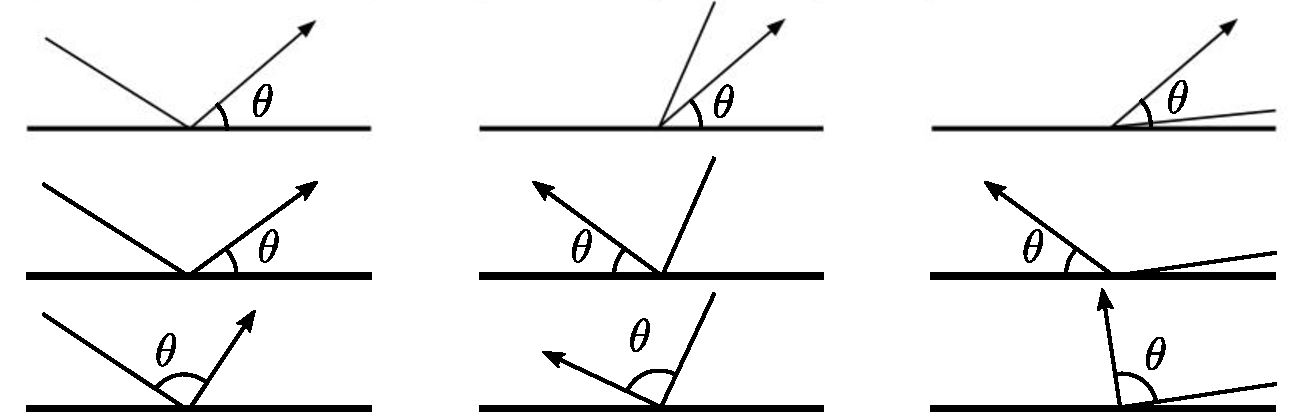
\includegraphics[width=0.8\linewidth]{figures/bounce_examples.pdf}
    \centering
    \caption[test]{\label{fig:bex}Examples of different ``bouncing laws" which can be implemented on
mobile robots. In the first row, $b(\alpha, \theta) = \theta$, which we refer to
as a \textbf{fixed} bounce law. In the second row, we have a \textbf{monotonic
fixed} bounce law, where
$b(\alpha, \theta) = \theta$ or $\pi-\theta$, depending on what is necessary to
preserve monotonicity of travel direction along the $x$-axis. In the third
row, $b(\alpha, \theta) = \alpha - \theta$, rotating $\alpha$ through $\theta$ in the clockwise
direction. It is possible that this rotation will cause the 
heading of the robot to still be facing into the boundary, in which case this model usually has the robot 
perform the rotation again until its heading points into the free space. We
refer to this as a \textbf{relative} bounce law ($\alpha$ appears on the
right hand side of the bounce law).
}
\end{figure}

\begin{definition}
Let $\alpha: (0,\pi)$ be the robot's incoming heading relative to the
environment boundary. A \textbf{bounce law} $b$ maps $\alpha$ to an action
$u$, and determines how the robot will reorient itself when it collides with a
boundary. Bounce laws are defined in the
frame where the environment normal is aligned with the positive $y$ axis and the
robot's point of contact with the wall is the origin. 
\end{definition}

For example, a specular bounce (laser beams, billiard balls) has bounce law
$b(\alpha) = \pi - \alpha$. See Figure \ref{fig:bex} for more
example bounce laws. 

\begin{definition}
A \textbf{bounce strategy} is a deterministic finite state machine where each
state indicates a certain (possibly nondeterministic) bounce law, and the input language is that of the
robot's sensor readings.
\end{definition}

Given a polygonal environment (such as the floor plan of a warehouse or office
space), we would like to synthesize bounce strategies which allow a robot to
perform a given task (such as navigation, patrolling, or localization).


\section{Visibility-Based Boundary Partitioning} \label{sec:partition}

\begin{definition}
The \textbf{visibility polygon} of a point $s$ in a polygon $P$ is the polygon
formed by all the points in $P$ which can be connected to $s$ with a line
segment which lies entirely within $P$.
\end{definition}

Imagine a robot sliding along the boundary of a polygon, calculating 
the visibility polygon as it moves. In a convex polygon, nothing exciting 
happens, but in a nonconvex polygon, the reflex vertices (vertices with an
internal angle greater than $\pi$) cause interesting
behavior.

As the robot slides, its visibility polygon may change continuously: edges
shrink or grow, but the combinatorial structure of the polygon remains the same.
However, when the robot aligns with a reflex vertex $r$ and another vertex $v$ (visible
from $r$), a combinatorial change will occur in the visibility polygon. Either 
$v$ will become visible to the robot, adding an edge to the visibility 
polygon, or $v$ will disappear behind $r$, removing an edge from the visibility polygon.

To compute all such points where the visibility polygon changes structure, we
must compute the \textbf{partial local sequence}, defined in \cite{rourke_viz}.
The partial local sequence is a sequence of vertices, associated with a vertex
$v_0$ in $P$, such that we shoot a ray through $v_0$ from every vertex in $P$
that is visible from $v_0$ and keep the resulting sequence of intersections with
$\partial P$. If $v_0$ is reflex, some of the rays shot through it may intersect
$\partial P$ in the interior of existing edges. See Figure \ref{fig:pls} for an
example of the vertices in the partial local sequence of $v_0$ (blue dots with
accompanying rays).

Thus, once all the partial local sequences have been inserted into the original
polygon, the resulting intervals along the boundary define a set of equivalence
classes, where two points in the same interval can see the same edge set of the
original polygon (though they may see different portions of those edges). Thus,
we can reason over a finite set of transitions between these intervals, instead
of the infinite set of possible transitions between points on the boundary of
the original polygon. See Algorithm \ref{algo:insert} for a pseudocode
description of this partitioning process.

Let $P'$ be the polygon $P$ with all partial local sequence points inserted.
Let the edge set of $P'$ be $E'$, with $n'$ elements.

\begin{definition}
The \textbf{edge visibility graph} of a polygon $P$ has a node for each edge of
$P$, and has an arc between two nodes $(e_i, e_j)$ if and only if there is a
point $s_i$ in the open edge $e_i$ and a point $s_j$ on the open edge $e_j$ such
that $s_i$ and $s_j$ can be connected with a line segment which is entirely
within the interior of $P$.
\end{definition}

\begin{definition}
Let $\thicksim$ be an equivalence relation such that for $s_1, s_2 \in \partial
P$, $s_1 \thicksim s_2$ if and only if the visibility polygons of $s_1$ and $s_2$ have
the same edge visibility graphs.
\end{definition}

This relation satisfies the necessary
properties {\color{red} todo but easy},

\begin{itemize}
\item reflexivity
\item symmetry
\item transitivity
\end{itemize}

The partition of $\partial P$ created by Algorithm \ref{algo:insert} are the
equivalence classes induced by $\thicksim$ {\color{red} todo but easy}.


\begin{definition}
Let the \textbf{bounce visibility graph} be the directed edge visibility graph of
$P'$.
\end{definition}

While visibility is a symmetric property, we use directed edges so that 
we can augment each edge with a label function which stores
geometrical constraints on the visibility from one edge to another, which are
not symmetric and govern what actions the robot can take from one edge to
reach another. See Section \ref{sec:safe} for further exploration of this idea.


We now define the \textbf{bounce visibility diagram}, which is a
representation of the edge-edge visibility of a polygon $P'$. This representation
was inspired by link diagrams \cite{efrat2000sweeping,tan_sweep}, though our
diagrams represent only a link distance of one.
%We choose an arbitrary vertex
%$v_0$ of $P$ as the origin, and parameterize points $p \in \partial P$ by the
%counterclockwise distance from $v_0$, divided by the perimeter length of
%$\partial P$. This parameterization defines a bijective function $s: [0,1) \to \partial P$.
If $|\partial P'|$ is the perimeter length of $\partial P'$, let the $x-$axis of the
bounce visibility diagram be the interval $[0, |\partial P'|)$, where the
endpoints of the interval are identified. Let the $y-$axis of the diagram be a
parameter $\theta$ which is an angle between $0$ and $\pi$.
We also use a labelling function $\ell: \partial P' \to [0, \ldots, n']$ to
label each point $p \in \partial P'$ with the edge segment in $P'$ that it
belongs to. Thus, for a point $s \in \partial P'$, and an angle $\theta$, we can
compose $\ell$ and the state transition function $f$ to compute
$l(f(s,\theta))$. The graph of $l \circ f$ is the bounce visibility diagram: 
the diagram indicates which edge
of $\partial P'$ is visible from points along $\partial P'$, and at which angle
ranges, which correspond to actions the robot could take from that point.

{\color{red} change so regions are assigned a unique "color" or "label" based on
destination segment, and get plots to reflect this}

The bounce visibility diagram gives us some visual insight into the structure of
the problem. For example, in Figure \ref{fig:regular_pent_bvd} we can see that
there are intervals of $\theta$ for which we can draw lines horizontally across
the diagram while only crossing vertical lines (indicating changes in visibilit
y at a vertex). If we can draw such lines across the region of a single
segment, it indicates that for that range of $\theta$, all bounces departing at
that angle from anywhere in the segment will land on the same segment. If we can
draw such lines across the entire diagram, this indicates that this property
holds true for the entire polygon. We call such transitions \emph{safe
actions}, since for a range of $\theta$, $f(s,\theta)$ maps from one equivalence
class on the boundary to another without splitting the $s$-interval.

{\color{red} need nice example here, something a little more exciting than
regular pentagon, maybe two convex shapes with hallway between}

\begin{figure}[h]
\centering
\begin{subfigure}{0.4\textwidth}
    \centering
    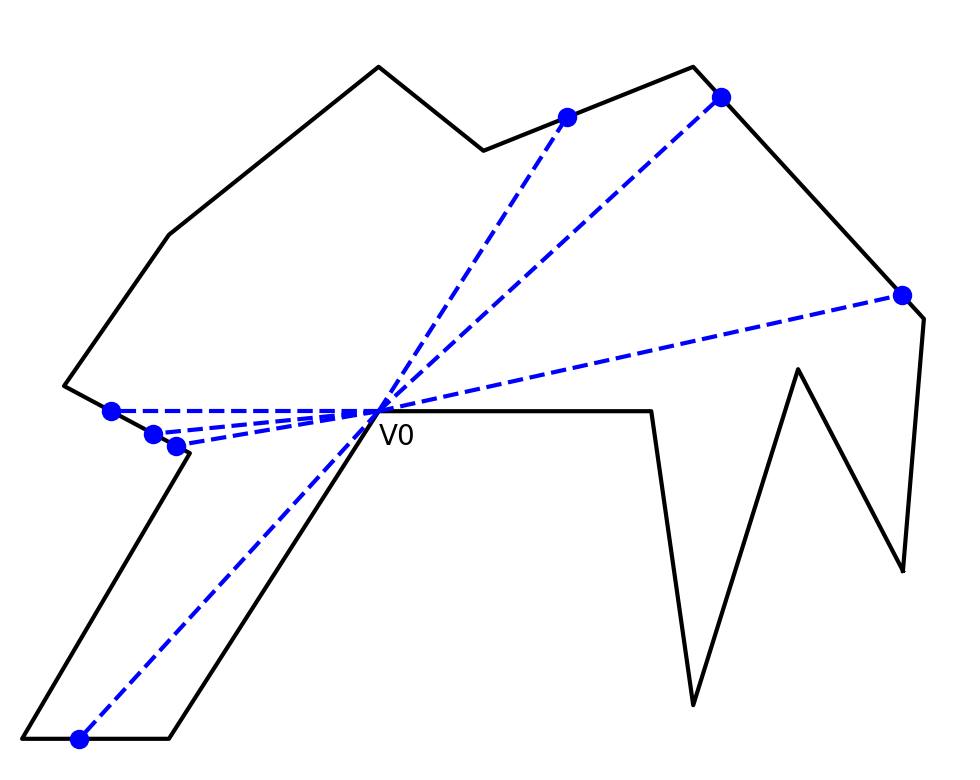
\includegraphics[width=\linewidth]{figures/partial_local_sequence.png}
    \caption{Partial local sequence for $v_0$}\label{fig:pls}
\end{subfigure}%
\begin{subfigure}{0.4\textwidth}
    \centering
    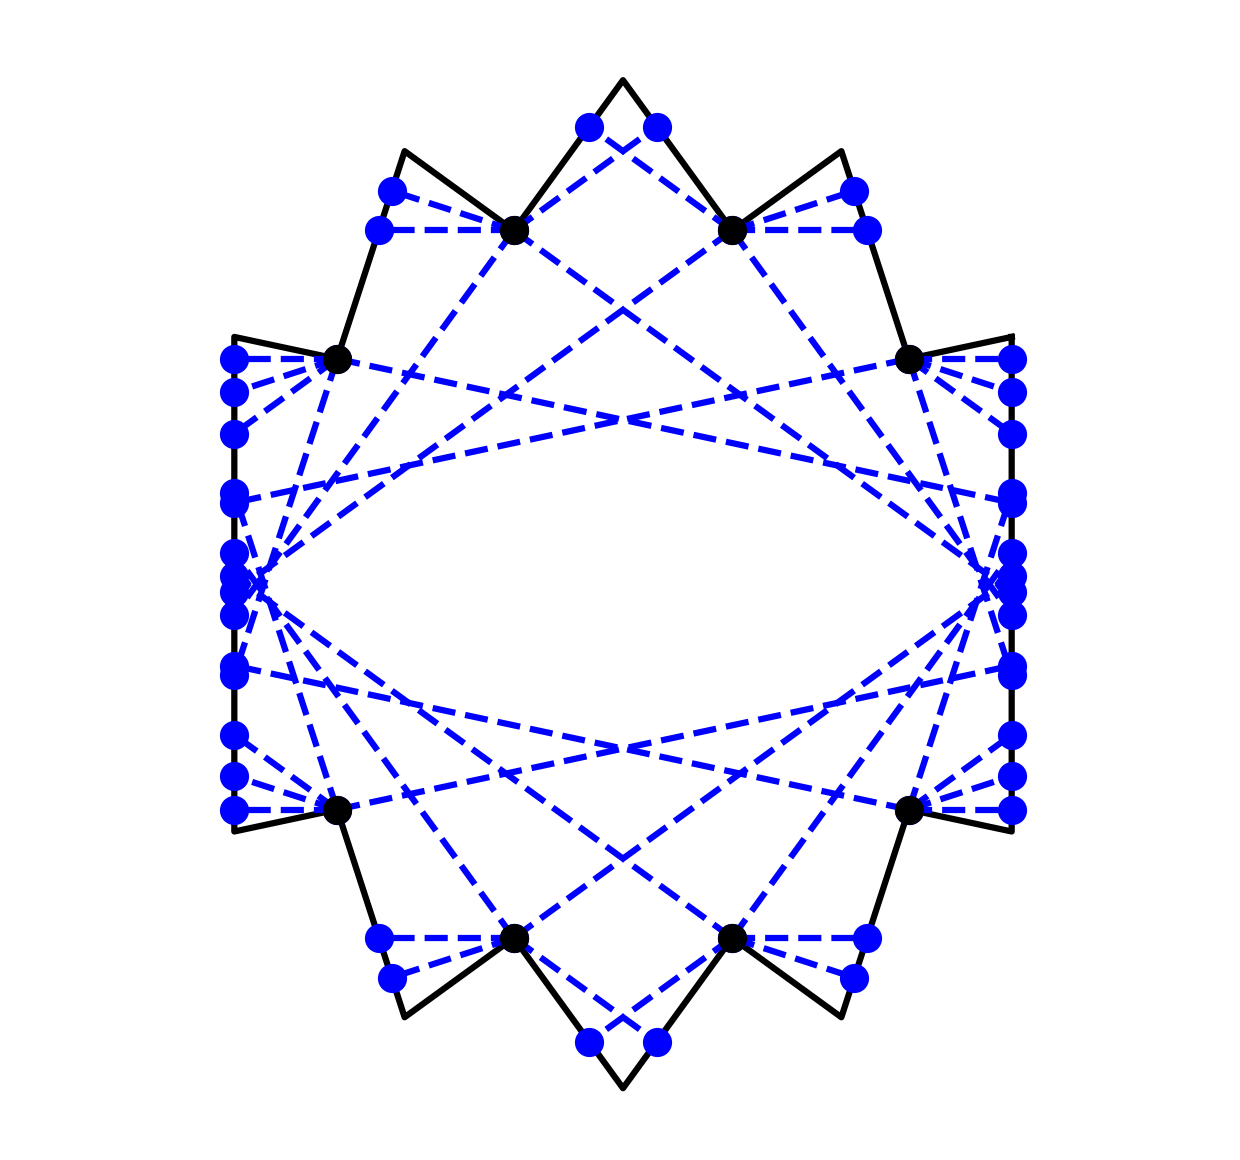
\includegraphics[width=\linewidth]{figures/chestnut_5.png}
    \caption{The worst case polygon for $t=4$. \label{fig:t4}}
\end{subfigure}
\end{figure}

\begin{algorithm}
\caption{Partition the boundary of a polygon into visibility
equivalence classes.}
\label{algo:insert}
\begin{algorithmic}
\Procedure{PartitionPoly}{$poly$}
\State $v_{new} \gets \{\}$
\State $reflex\_verts \gets$ \Call{GetReflexVerts}{$poly$}
\For{$v_r$ in $reflex\_verts$} \Comment{visible vertices from reflex vertex induce transitions}
    \For{$v_{vis}$ in \Call{VisibleVerts}{$poly, v_r$}} 
        \State $v_{new} \gets$ $v_{new} \cup$ \Call{ShootRay}{$v_{vis}, v_r$}
    \EndFor
\EndFor
\State $partitioned\_poly \gets$ \Call{InsertVerts}{$v_{new}, poly$}
\State \textbf{return} $partitioned\_poly$
\EndProcedure
\end{algorithmic}
\end{algorithm}

\begin{proposition} The bounce visibility graph for a polygon with $n$ vertices has 
$O(n^2)$ vertices and $O(n^4)$ edges.
\end{proposition}

\begin{proof}

Consider a polygon $P$ with $n$ vertices, $r$ of which are reflex vertices. To
construct the bounce visibility graph, we insert the vertices of the partial
local sequence for each vertex in $P$. For a convex vertex, its partial local sequence 
will not add any new vertices to $P$. However, a reflex vertex can add $O(n)$ new vertices. 

Up to half of the vertices in the polygon can be reflex, so the complexity of
$r$ is $O(n)$. Therefore, the number of vertices in $P'$, returned by Algorithm
\ref{algo:insert} is $O(n^2)$. Each vertex corresponds to an edge in $P'$, and
thus a node in the edge visibility graph of $P'$. At most, a given vertex in $P'$ may see all other vertices, so in the worst
case, the bounce visibility graph will have $O(n^4)$ edges.
\qed

\end{proof}

\subsubsection{Worst Case Example}

We might hope that if $r$ is large, then not all of the reflex vertices will
produce a large number of new vertices, and we may bound the size of the edge
set in the visibility graph. Unfortunately, the number of reflex
vertices, the new vertices produced in their partial local sequence, and the new
vertices' visibility can be large at the same time. We will present a family of
input polygons with bounce visibility graph edge-set size of $O(n^4)$.

Let $n = 4t+2$, where $t$ is a positive integer. We design a polygon with
$r = 2t$ reflex vertices. The polygon is symmetric with respect to its medium
horizontal line. In the top half, the reflex vertices are uniformly located on a
circle and thus they are visible to each other; the convex vertices are chosen
so that they are outside the circle and the line through an edge will not
intersect other edges. Each reflex vertex will have at least $t-1$ new
vertices in its partial local sequence. There will be $2t(t-1)+n$
vertices in the polygon after we insert all new vertices in the partial local
sequence for all reflex vertices. Each of them can see at least $t(t-1)+n/2$
other vertices. Thus the number of edges in the transition graph for the
polygon with inserted vertices is
$O ((2t(t-1)+n)(t(t-1)+n/2)) = O(t^4) = O(n^4)$.
Fig \ref{fig:t4} shows the polygon for $t = 4$ with all the
vertices in the partial local sequences. % show the diagram to edge


%\begin{figure}
%
%\centering
%\begin{subfigure}{0.35\textwidth}
%\centering
%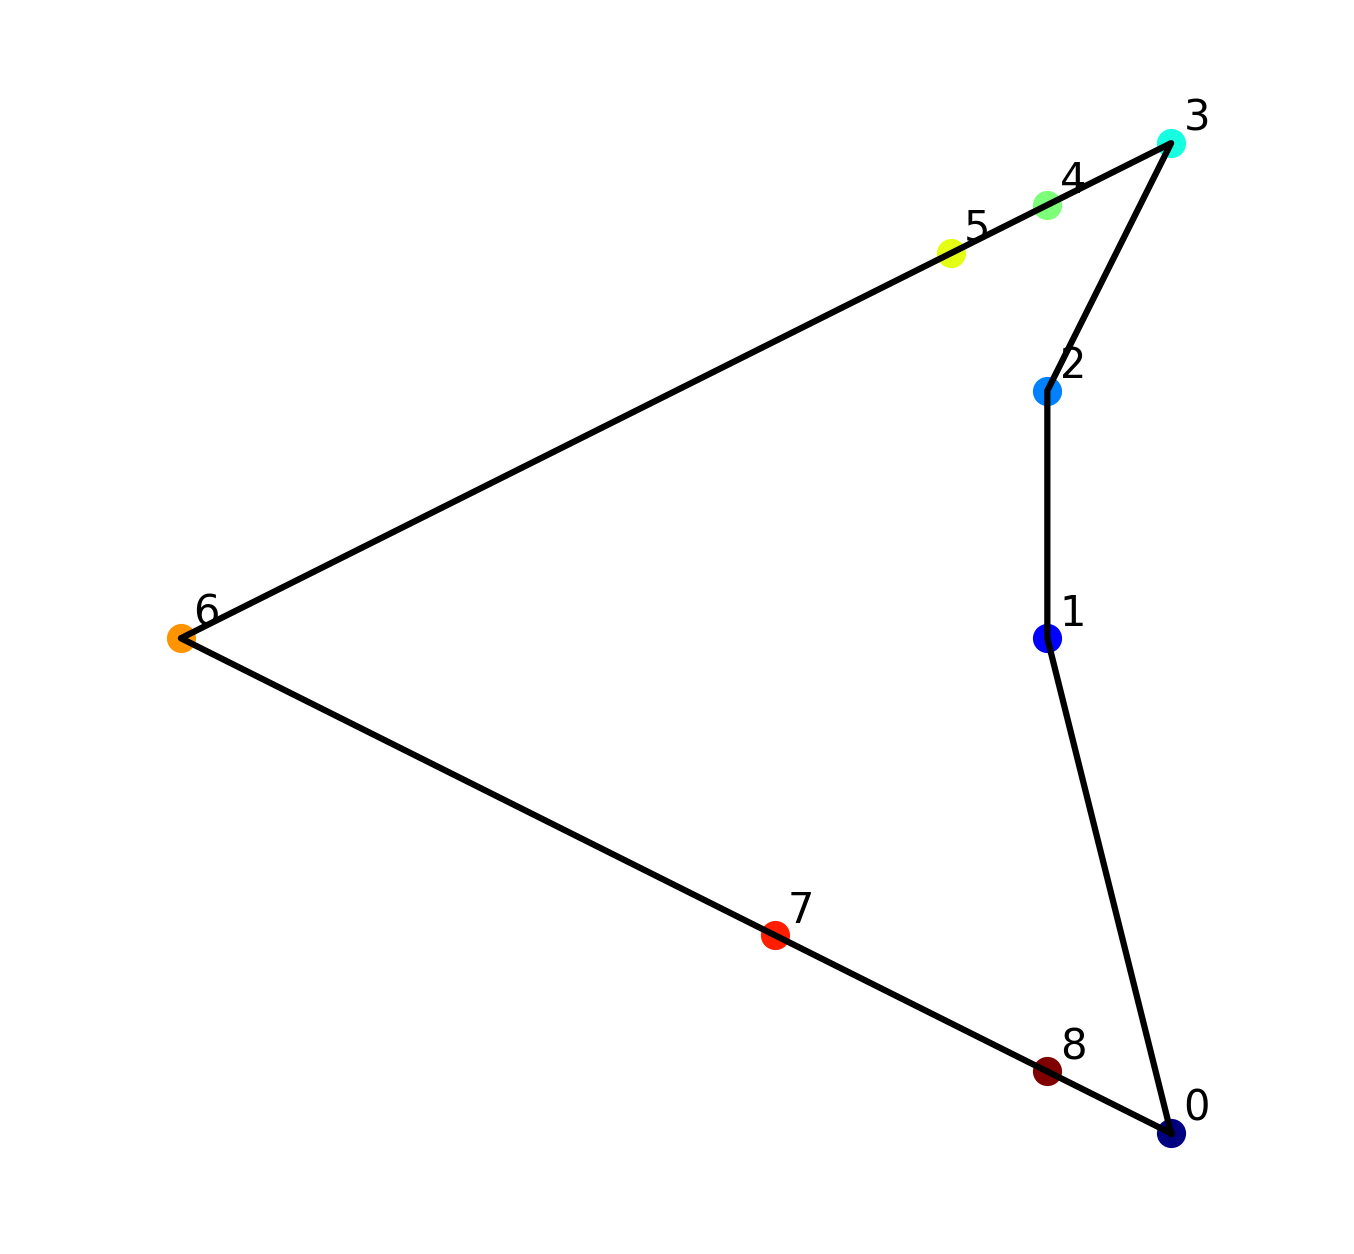
\includegraphics[width=\linewidth]{figures/color_pent.png}
%\captionof{figure}{\label{fig:color_pent}}
%\end{subfigure}%
%\begin{subfigure}{0.35\textwidth}
%\centering
%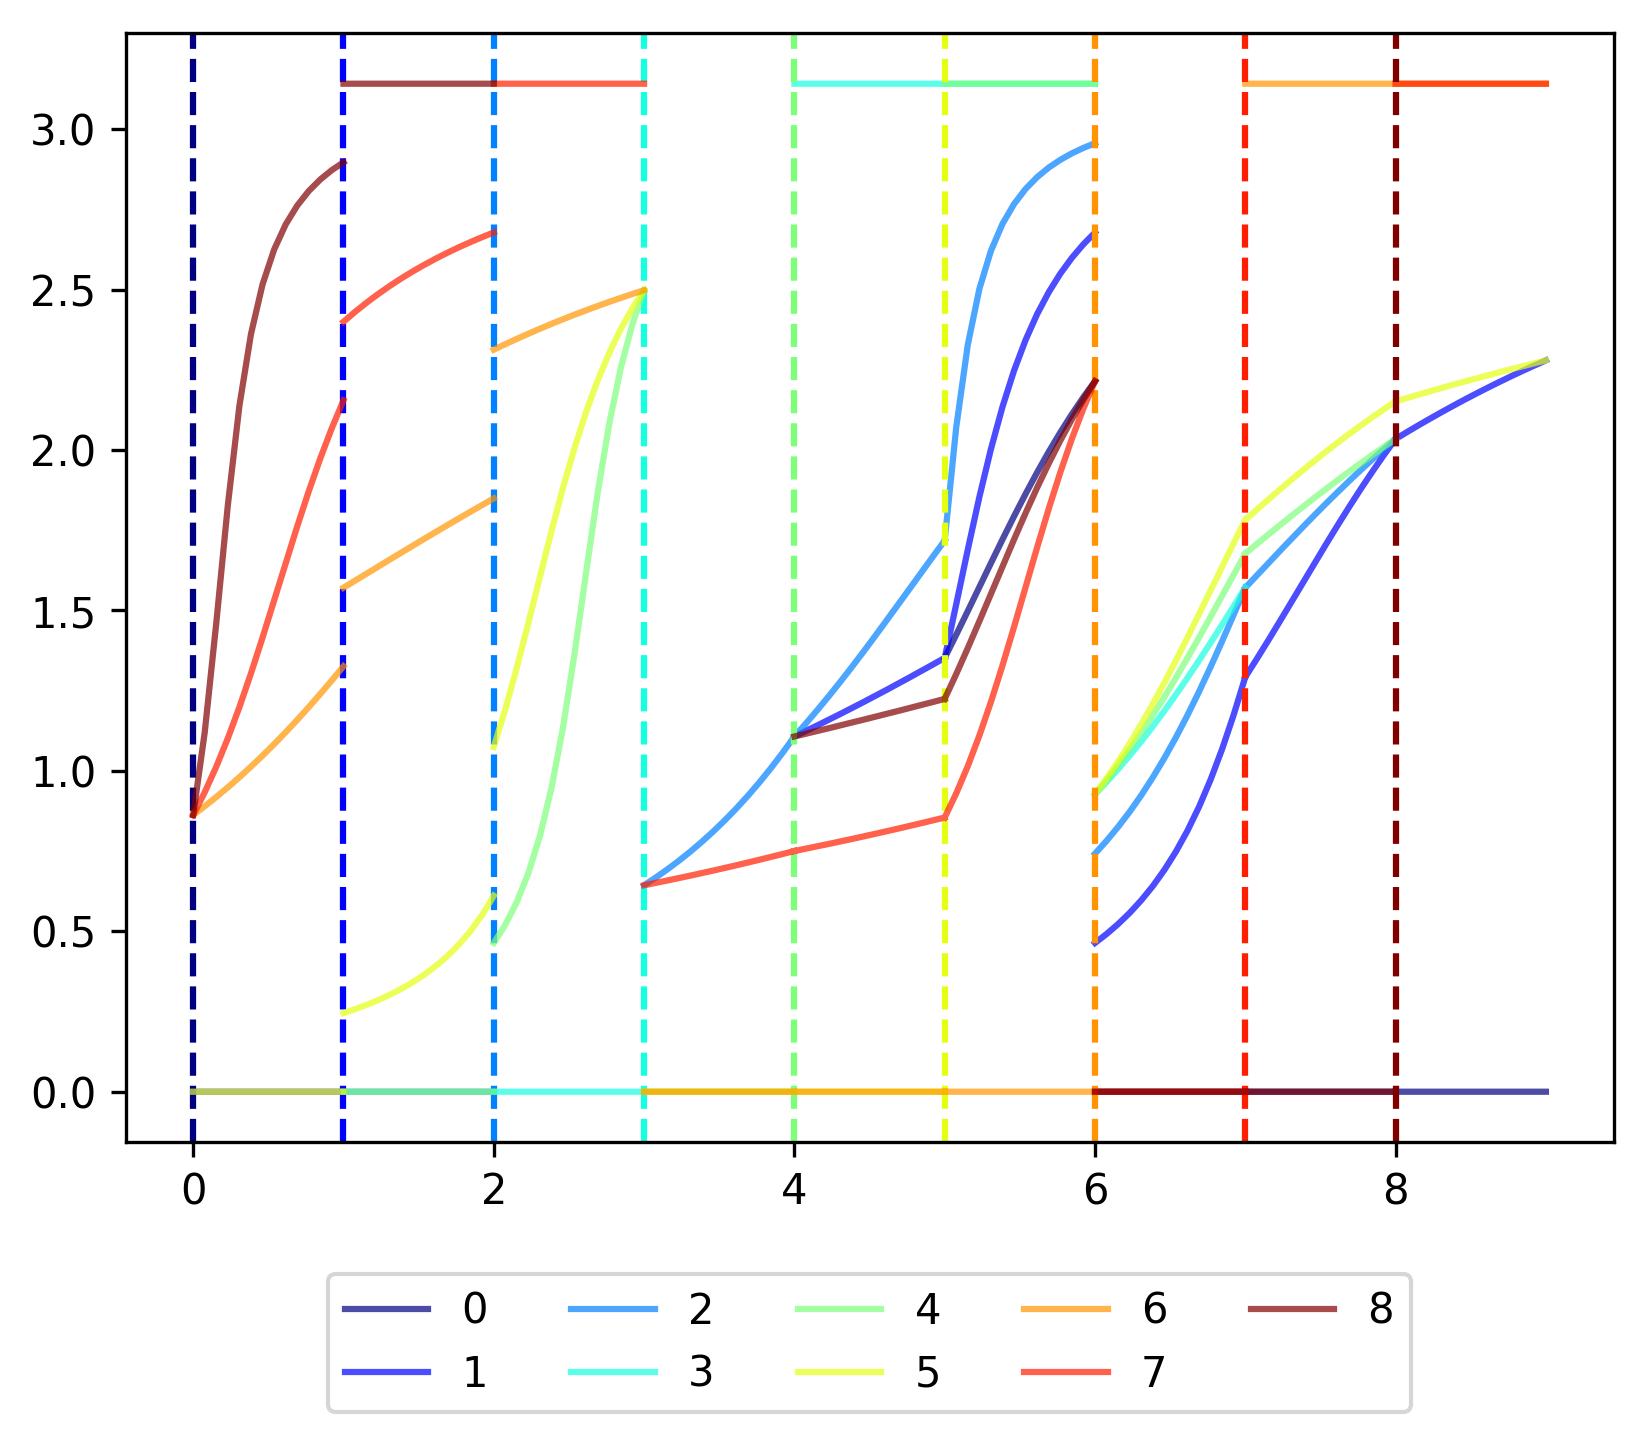
\includegraphics[width=\linewidth]{figures/bvd.png}
%\end{subfigure}
%\caption{A polygon and its corresponding bounce visibility diagram.}
%\label{fig:bvd}
%\end{figure}
%
%\begin{figure}
%\centering
%\begin{subfigure}{0.35\textwidth}
%\centering
%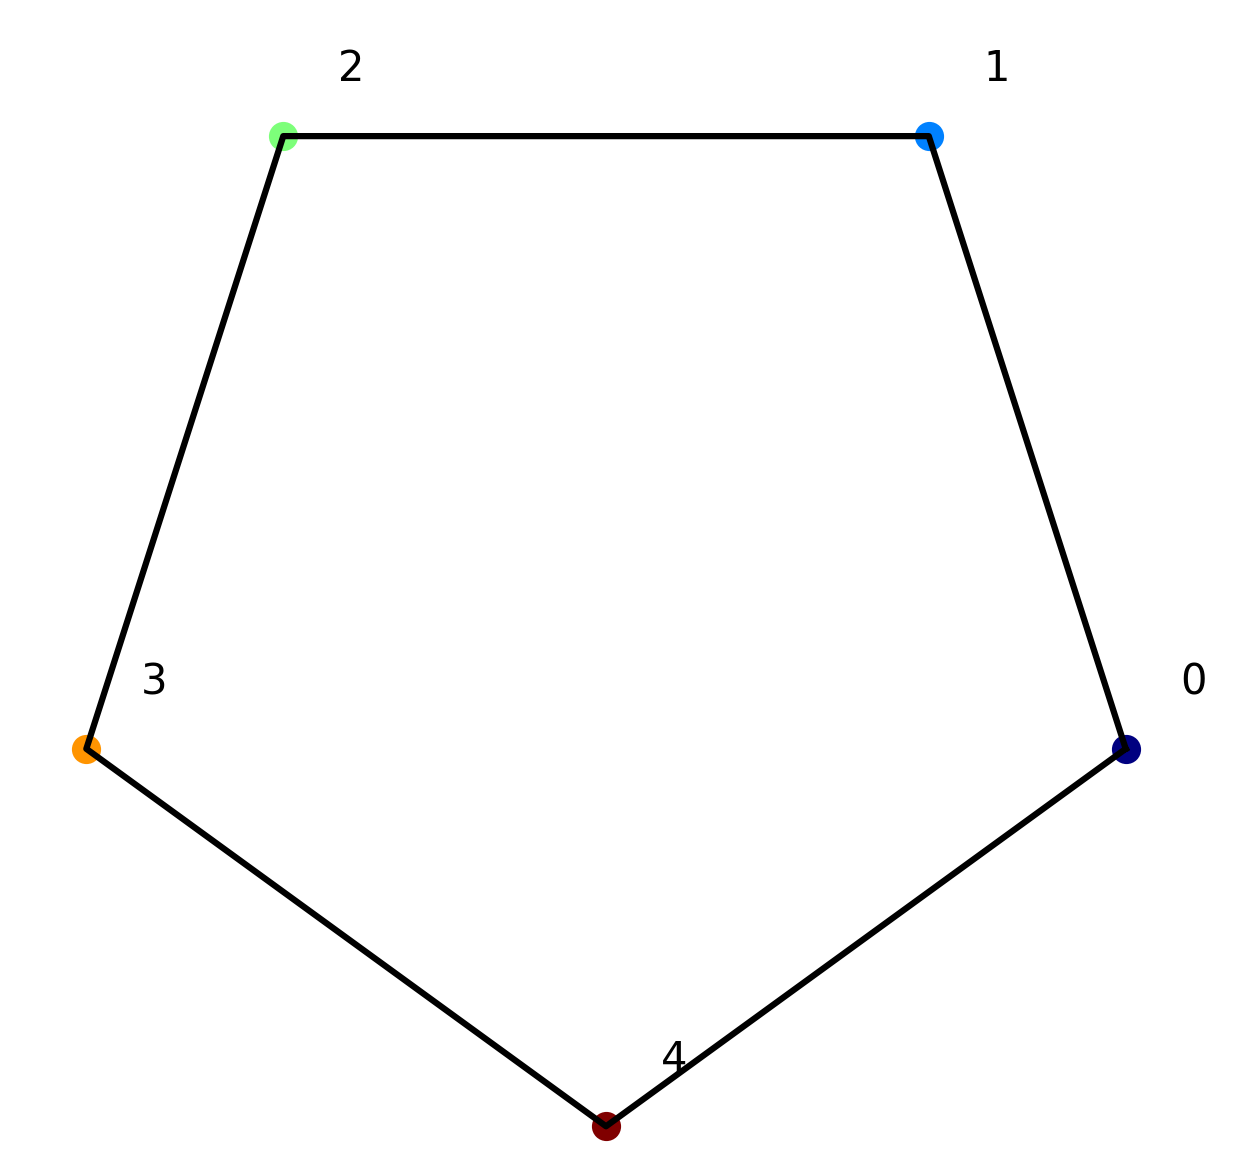
\includegraphics[width=\linewidth]{figures/regular_pent.png}
%\end{subfigure}%
%\begin{subfigure}{0.35\textwidth}
%\centering
%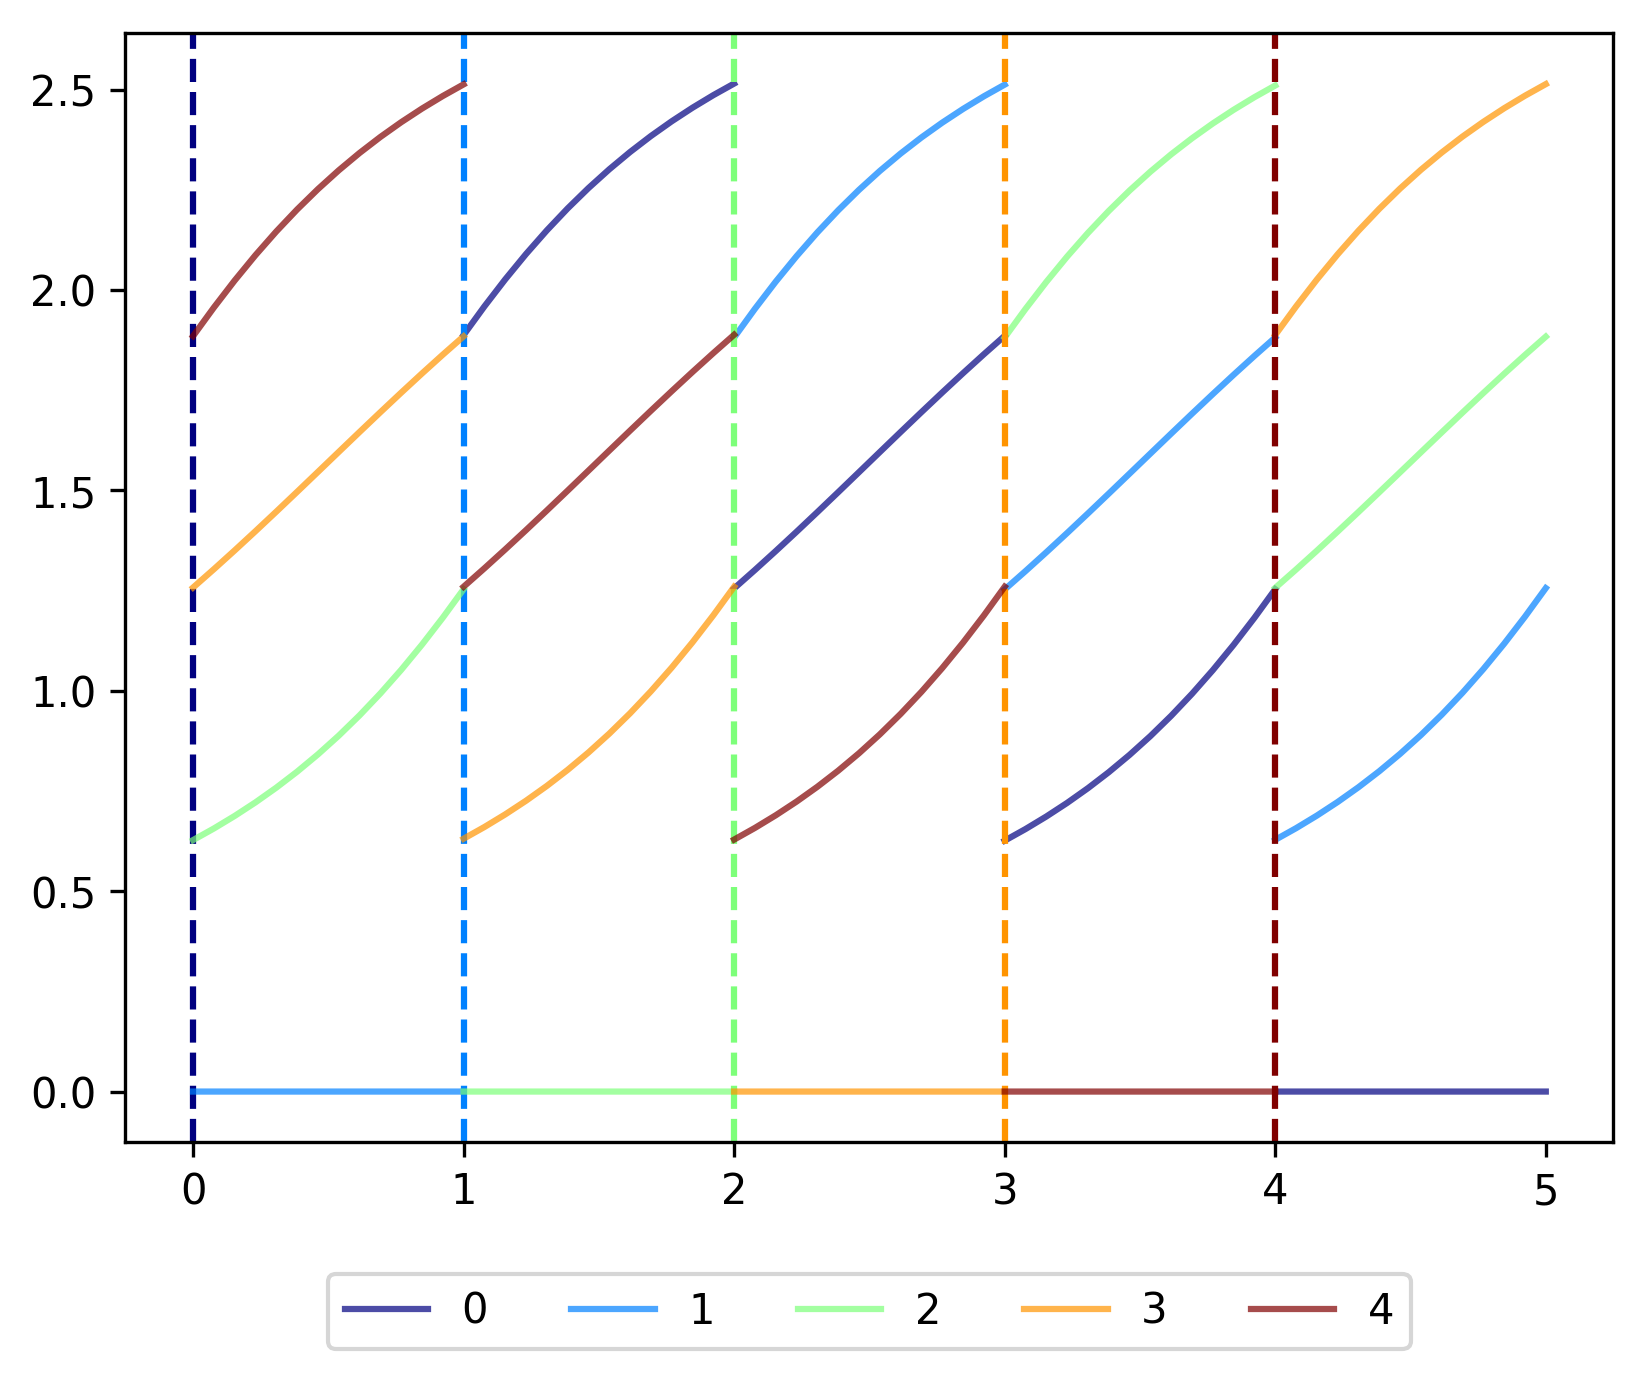
\includegraphics[width=\linewidth]{figures/regular_pent_bvd.png}
%\end{subfigure}
%\caption{The bounce visibility diagram for the regular pentagon. }
%\label{fig:regular_pent_bvd}
%\end{figure}

\section{Combinatorial Path Families}

{\color{red} Introduce running example - floor plan with three features: region
of high symmetry (maybe a row of offices), region with nonconvexity, and long
hallway.

Show with examples how useful trajectories in example correspond to queries to
the graph.}

One major advantage of this approach is that it allows us to characterize
properties of families of paths the robot may take. For example, the  
two paths in Figure \ref{fig:twopaths} are produced by different sequences of
bounces, but have the same sequence of edge collisions and have the same overall
dynamical behavior (escape the room on the left, travel through hallway, then
patrol the room on the right in a periodic orbit).

\begin{figure}
\centering
\begin{subfigure}{0.5\textwidth}
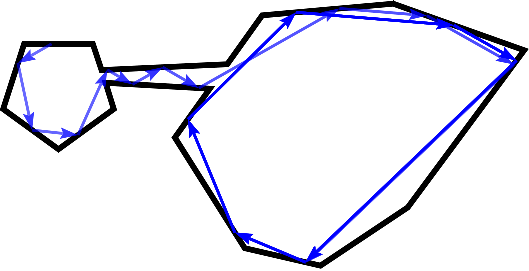
\includegraphics[width=\linewidth]{figures/twoc_a}
\end{subfigure}%
\begin{subfigure}{0.5\textwidth}
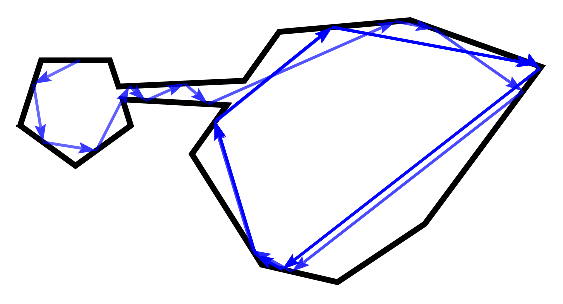
\includegraphics[width=\linewidth]{figures/twoc_b}
\end{subfigure}
\caption{Two paths belonging to the same combinatorial family.}
\label{fig:twopaths}
\end{figure}

To characterize some of these families of paths, we will use the boundary
partition technique defined in Section \ref{sec:partition}, then define
\emph{safe actions} between segments in the partition, where safe actions are
ones which are guaranteed to be successful from anywhere in a segment under an
interval of bounce angles.

\begin{definition}
Two edges $i,j \in \partial P$ are \textbf{entirely visible} to each other if
and only if every pair of points $x \in i$ and $y \in j$ are visible (the
shortest path between $x$ and $y$ in entirely within $P$).
\end{definition}

\begin{proposition}
Given two entirely visible line segments $i$ and $j$, it is possible to compute
the maximum range of angles $\tilde{\theta}_{max} = [\theta_r, \theta_l]$ such
that $f(s, \theta) \in j$, for all $s \in i$ and for all
$\theta \in \tilde{\theta_{max}}$, or we may compute that no such range exists.
\end{proposition}

\begin{proof}

Let edge $i = (v_i, v_{i+1})$ be aligned with the positive $x$ axis with the clockwise
endpoint at the origin, without loss of generality. Due to the edges being
entirely visible, $j = (v_j, v_{j+1})$ must be in the top half of the plane, above $i$.

Take the quadrilateral formed by the convex hull of the edge endpoints.
Let the edges between $i$ and $j$ be $l = (v_i, v_{j+1})$ and the right-hand edge 
$r = (v_{i+1}, v_j)$. Let $\theta_{l}$ be
the angle between $l$ and the positive $x$ axis ($0 < \theta_l < \pi$); similarly
for $r$ and $\theta_r$. See Figure \ref{fig:bounce_range} for an illustration of
the setup. 

There are three cases to consider: if $l$ and $r$ are extended to infinity,
they cross either above or below edge $i$, or they are parallel.

\emph{Case 1:} $l$ and $r$ would meet below edge $i$. Then,
$\theta_l > \theta_r$ and if a ray is cast from any point on $i$ at angle
$\theta \in [\theta_r, \theta_l]$, the ray is guaranteed to intersect $j$ in its
interior.

\emph{Case 2:} $l$ and $r$ would meet above edge $i$. Then, $\theta_l <
\theta_r$, and there is no angle
$\theta$ such that a ray shot from \emph{any} point on $i$ will intersect $j$.
To see this, imagine sliding a ray at angle $\theta_l$ across the quadrilateral
- at some point before reaching $v_{i+1}$, the ray must stop intersecting $j$,
else we would have $\theta_l > \theta_r$.

\emph{Case 3:} $l$ and $r$ are parallel. This implies that $\theta_{l} =
\theta_{r}$, which is the only angle for which a transition from any
point on $i$ is guaranteed to intersect $j$, and $\tilde{\theta}_{max}$ is a
singleton set.

Thus, for each case, we can either compute the maximum angle range or determine
that no such angle range exists.
\qed

\end{proof}

Cases 1 and 3 correspond to our definition of a \emph{safe actions}.

\begin{definition}
A \textbf{safe action} between segments $i$ and $j$ is an action $u \in \tilde{\theta}_{max}$
, which requires $\tilde{\theta}_{max}$ for transition $i$ to $j$ is nonempty.
The resulting transition $f(s, \theta)$ is guaranteed to
go from $i$ to $s$ for any $s \in i$ and $\theta \in \tilde{\theta}_{max}$.
\end{definition}

Note that this definition is very similar to the definition of an interval of
safe actions from \cite{LewOKa13}.

\begin{lemma}
If two segments are entirely visible to each other, there will be at least one safe
action between them.
\end{lemma}

\begin{lemma}
If two segments share a vertex which is not reflex, there exist safe actions
from one to the other in both directions.
\end{lemma}

\begin{lemma}
For some polygons, not all segments in the partitioned polygon $P'$ are visible
from some other segment in $P'$.
\end{lemma}

{\color{red} define combinatorial families of paths}


%\begin{definition}\label{def:transition}
%For edge $e_{ij} \in E(G)$, for each point $x$ in the edge $i$, there 
%exists a range of angles $\tilde{\theta}$ such that $f(x,\theta) \in j$ for
%some $\theta \in \tilde{\theta}$.
%\end{definition}
%
%\begin{proof}
%By construction, edge $e_{ij}$ exists if and only if there is a point $x$ on the (open)
%segment $i$ and a point $y$ on the (open) segment $j$ such that $x$ and $y$ are
%visible to each other. Since $y$ is in the open segment, there will always be some $\epsilon$-neighborhood around
%$y$ which is also visible from $x$, and the endpoints of this
%$\epsilon$-neighborhood define a range of angles at which the robot may leave
%$x$ and arrive on segment $j$.
%
%This angle range can be constructed through simple trigonometry for a
%given point and target segment.
%\end{proof}

%\begin{definition} \label{def:angrange}
%Given two mutually visible segments $i,j \in \partial P$, there exists a range 
%of angles from which a transition from $i$ to $j$ is possible from from some
%point in $i$ to some point in $j$.
%See Figure \ref{fig:bounce_range}. This interval, $[\theta_{min}, \theta_{max}]$, 
%is the union of the point-wise angle intervals described in Definition
%\ref{def:transition}.
%\end{definition}

\begin{figure}
%    \centering
%    \begin{subfigure}{0.5\textwidth}
%    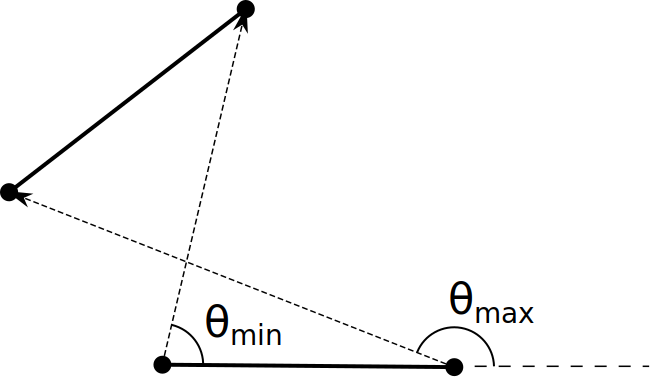
\includegraphics[width=0.4\linewidth]{figures/bouncerange.png}
%    \caption{Angle range such that a transition exists for some point on
%orginating edge.}
%\label{fig:bounce_range}
%    \end{subfigure}%
%    \begin{subfigure}{0.5\textwidth}
    \centering
    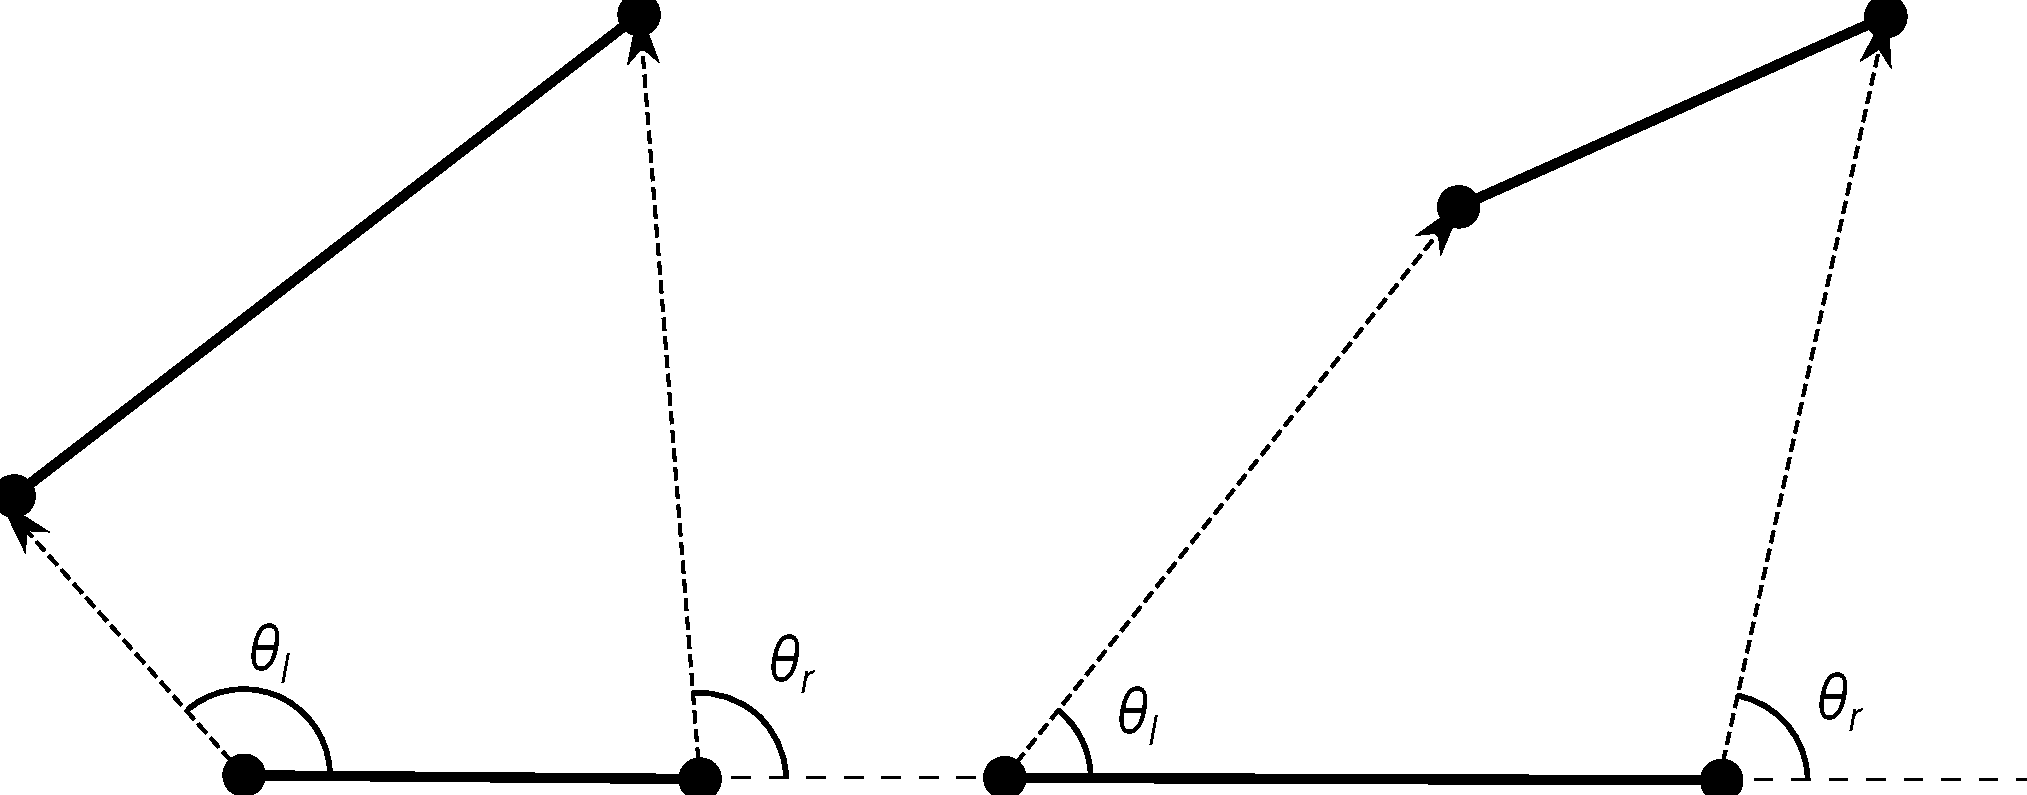
\includegraphics[width=0.7\linewidth]{figures/bouncerange_min.pdf}
    \caption{Angle range such that a transition exists for all points on
originating edge (left: such a range exists, right: such a range does not
exist)}
\label{fig:bounce_range}
%    \end{subfigure}
\end{figure}

\section{Dynamical Properties of Paths}

Many tasks required of mobile robots can be specified in terms of properties of
the path the robot takes through space. \emph{Navigation} requires a path that
begins and ends in specified regions; \emph{patrolling} requires a repeatable
path that satisfies some coverage criterion; \emph{localization} requires a path
which reduces uncertainty in the robot's position.

Our motion strategy allows us to disregard the robot's motion in the interior of
$P$. Instead, the robot's state is an interval (or possibly, set of intervals)
along the boundary $\partial P$, and we can formulate transitions as a discrete
dynamical system under the transition function $f$. 

A generally useful property of transitions between boundary segments is when the
transition is a \emph{contraction mapping}: two points, when mapped through the
transition, always become closer together. We can use this property to control
uncertainty in the robot's position, and to engineer stable limit cycles in
Section \ref{sec:cycles}.

\begin{definition}
Let $\phi_{ij}$ be the interior angle between two edges $i, j \in \partial P$ if
they are extended to infinity. The case where the segments are parallel will be
handled separately where necessary. 
\end{definition}

\begin{definition}

A function $f: \mathbb{R} \to \mathbb{R}$ is a contraction mapping if

\begin{equation*}
|f(x) - f(y)| \leq c |x-y|
\end{equation*}

where $0 \leq c < 1$. In other words, points under the mapping become closer
together.
\end{definition}
\begin{definition}
Suppose segment $i$ is aligned with $x$ axis with its normal pointing up and segment $j$ is above segment $i$. If the intersection of segment $i$ and $j$ is on the left of segment $i$, then call the transition from $i$ to $j$ a left transition; if the intersection is on the right of segment $i$, then call the transition a right transition.
\end{definition}

\begin{lemma} \label{lemma:angrange}
If the transition from segment $i$ to segment $j$ is a left transition, then the transition function $f(x, \theta)$ between segments $i$ and $j$ is a contraction mapping if and only if $\theta > \frac{\pi}{2}+\frac{\phi_{i, j}}{2}$; otherwise, the transition function $f(x, \theta)$ is a contraction mapping if and only if $\theta < \frac{\pi}{2}-\frac{\phi_{i, j}}{2}$.
\end{lemma}
\begin{proof}

\begin{figure}
    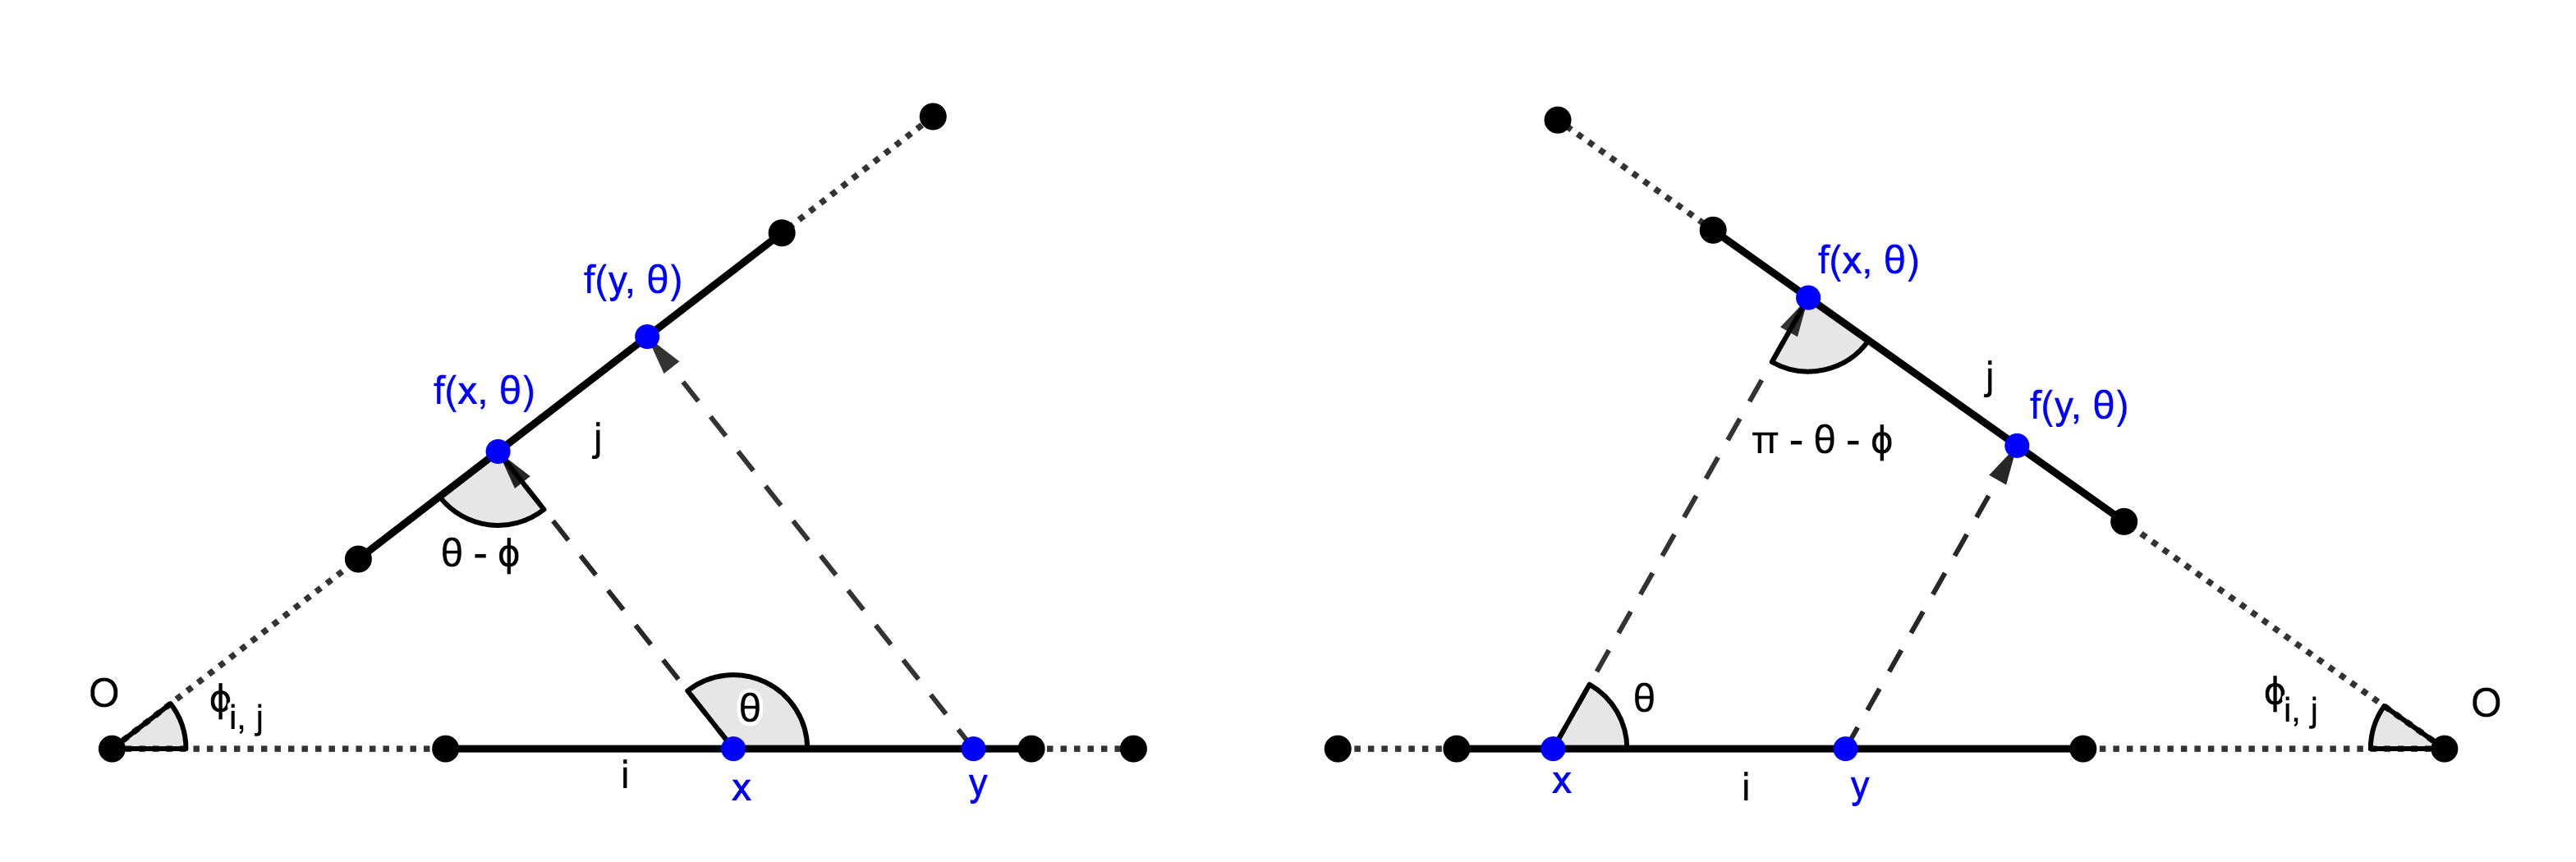
\includegraphics[width=1\linewidth]{figures/contraction_map_cond.png}
    \centering
    \caption{The two cases for computing contraction mapping conditions. \label{fig:cont_map}}
    \centering
\end{figure}

We consider the two cases of transition separately:
\begin{enumerate}
    \item For a left transition shown in the left diagram of figure~\ref{fig:cont_map}, \begin{eqnarray*}\overline{xf(x)} \parallel \overline{yf(y)} \Rightarrow \frac{|f(x)-f(y)|}{|x-y|} = \frac{|f(x)|}{|x|} = \frac{\sin(\pi - \theta)}{\sin(\theta - \phi_{i, j})} = \frac{\sin(\theta)}{\sin(\theta-\phi_{i, j})}.\end{eqnarray*} The transition will be contraction if and only if $\frac{|f(x)-f(y)|}{|x-y|} < 1 \iff \sin(\theta)<\sin(\theta-\phi_{i, j})$. If $\theta < \frac{\pi}{2}$, then $\sin(\theta) > \sin(\theta-\phi_{i, j})$. Thus we need $\theta>\frac{\pi}{2}$. If $\theta-\phi_{i, j} > \frac{\pi}{2}$, then $\sin(\theta) < \sin(\theta-\phi_{i, j})$ and we are done; otherwise we need $\pi - \theta < \theta-\phi_{i, j} \Rightarrow \theta - \frac{\phi_{i, j}}{2} > \frac{\pi}{2}$. Combining all conditions, we have the transition will be contraction if and only if $\theta >\frac{\pi}{2} + \frac{\phi_{i, j}}{2}$.
    \item Similarly, for a right transiton shown in the right diagram of figure~\ref{fig:cont_map}, \begin{eqnarray*}\overline{xf(x)} \parallel \overline{yf(y)} \Rightarrow \frac{|f(x)-f(y)|}{|x-y|} = \frac{|f(x)|}{|x|} = \frac{\sin(\pi - \theta)}{\sin(\pi -\theta-\phi_{i, j})} = \frac{\sin(\theta)}{\sin(\theta + \phi_{i, j})}.\end{eqnarray*} The transition will be contraction if and only if $\frac{|f(x)-f(y)|}{|x-y|} < 1 \iff \sin(\theta)<\sin(\theta+\phi_{i, j})$. If $\theta  > \frac{\pi}{2}$, then $\sin(\theta) > \sin(\theta + \phi_{i, j})$. Thus we need $\theta<\frac{\pi}{2}$. If $\theta+\phi_{i, j} < \frac{\pi}{2}$, then $\sin(\theta) < \sin(\theta+\phi_{i, j})$ and we are done; otherwise we need $\theta < \pi-\theta-\phi_{i, j} \Rightarrow \theta < \frac{\pi}{2} - \frac{\phi_{i, j}}{2}$. Combining all conditions, we have the transition will be contraction if and only if $\theta <\frac{\pi}{2} - \frac{\phi_{i, j}}{2}$.
\end{enumerate}
\qed

\end{proof}


\begin{definition}
Define $C(\theta, \phi_{i, j})$ as the \textbf{contraction coefficient} of a transition between two
edges $i$ and $j$ of $\partial P$. For a left transition, $C(\theta, \phi_{i, j}) = | \frac{\sin(\theta)}{\sin(\theta - \phi_{i, j})} |$; for a right transition,  $C(\theta, \phi_{i, j}) = | \frac{\sin(\theta)}{\sin(\theta + \phi_{i, j})} |$.
\end{definition}

For a sequence of bounces $b_1, \ldots, b_k$, we can construct the overall
mapping from the domain of $b_1$ to the range of $b_k$ through function
composition. Since $f$ is a linear mapping, the contraction property of a composition 
of multiple bounces can be determined by multiplying the contraction
coefficients.

If $\prod_{i=1}^k C(\theta_i, \phi_i) < 1$, the composition of bounces $b_1, \ldots, b_k$
is a contraction mapping. This is true even if some transition $b_i$ is not a
contraction mapping, since the coefficient is simply the ratio of distances
between points before and after the mapping is applied. Furthermore, the value
of $\prod_{i=1}^k C(\theta_i, \phi_i)$ tells us the exact amount by which the
size of the set of possible robot states has shrunk.

{\color{red} describe how to propagate angle constraints and contraction coeffs
over intervals of theta. Connect back to funnelling, maybe with a fig if we
have space}

%and the constraints on the angle range $\tilde{\theta}$ can be propagated through the 
%composition by intersecting the angle intervals.

\subsection{Cycles} \label{sec:cycles}

A very common use of contraction mappings is to prove the existence of fixed
points, due to the power of the Banach fixed point theorem \cite{Granas2003}.
The exact condition needed is for a contraction mapping to map an interval back
to itself. Since the transition function of a bouncing robot path is the
composition of the individual bounce transition functions, we can create such a
mapping by constructing a path which returns to its originating edge. A fixed
point of this mapping is a stable limit cycle, which can be used to reduce an
interval of possible robot positions to a single point (in the asymptotic
limit).

Such paths
in regular polygons were characterized in \cite{NilBecLav17}, but have been
observed experimentally in nonregular convex and nonconvex polygons. Here, we
present a more general proof for the existence of limit cycles in all convex
polygons.

\begin{definition}
If a limit cycle inside a convex polygons with $n$ edges forms another convex
polygon with $n$ edges, we call this limit cycle as convex $n$-cycle.
\end{definition}

\begin{definition}
$\phi_{P,min}$ is the smallest interior angle in a polygon $P$. We will omit the
label $P$ when it is clear from context.
\end{definition}

\begin{theorem} \label{thm:convex}
For all convex polygons with $n$ edges, there exists a range for $\theta$ such that fixed-angle bouncing strategy with $\theta$ will lead to a convex $n$-cycle regardless of the robot's start position.
\end{theorem}
\begin{proof}
\begin{figure}
    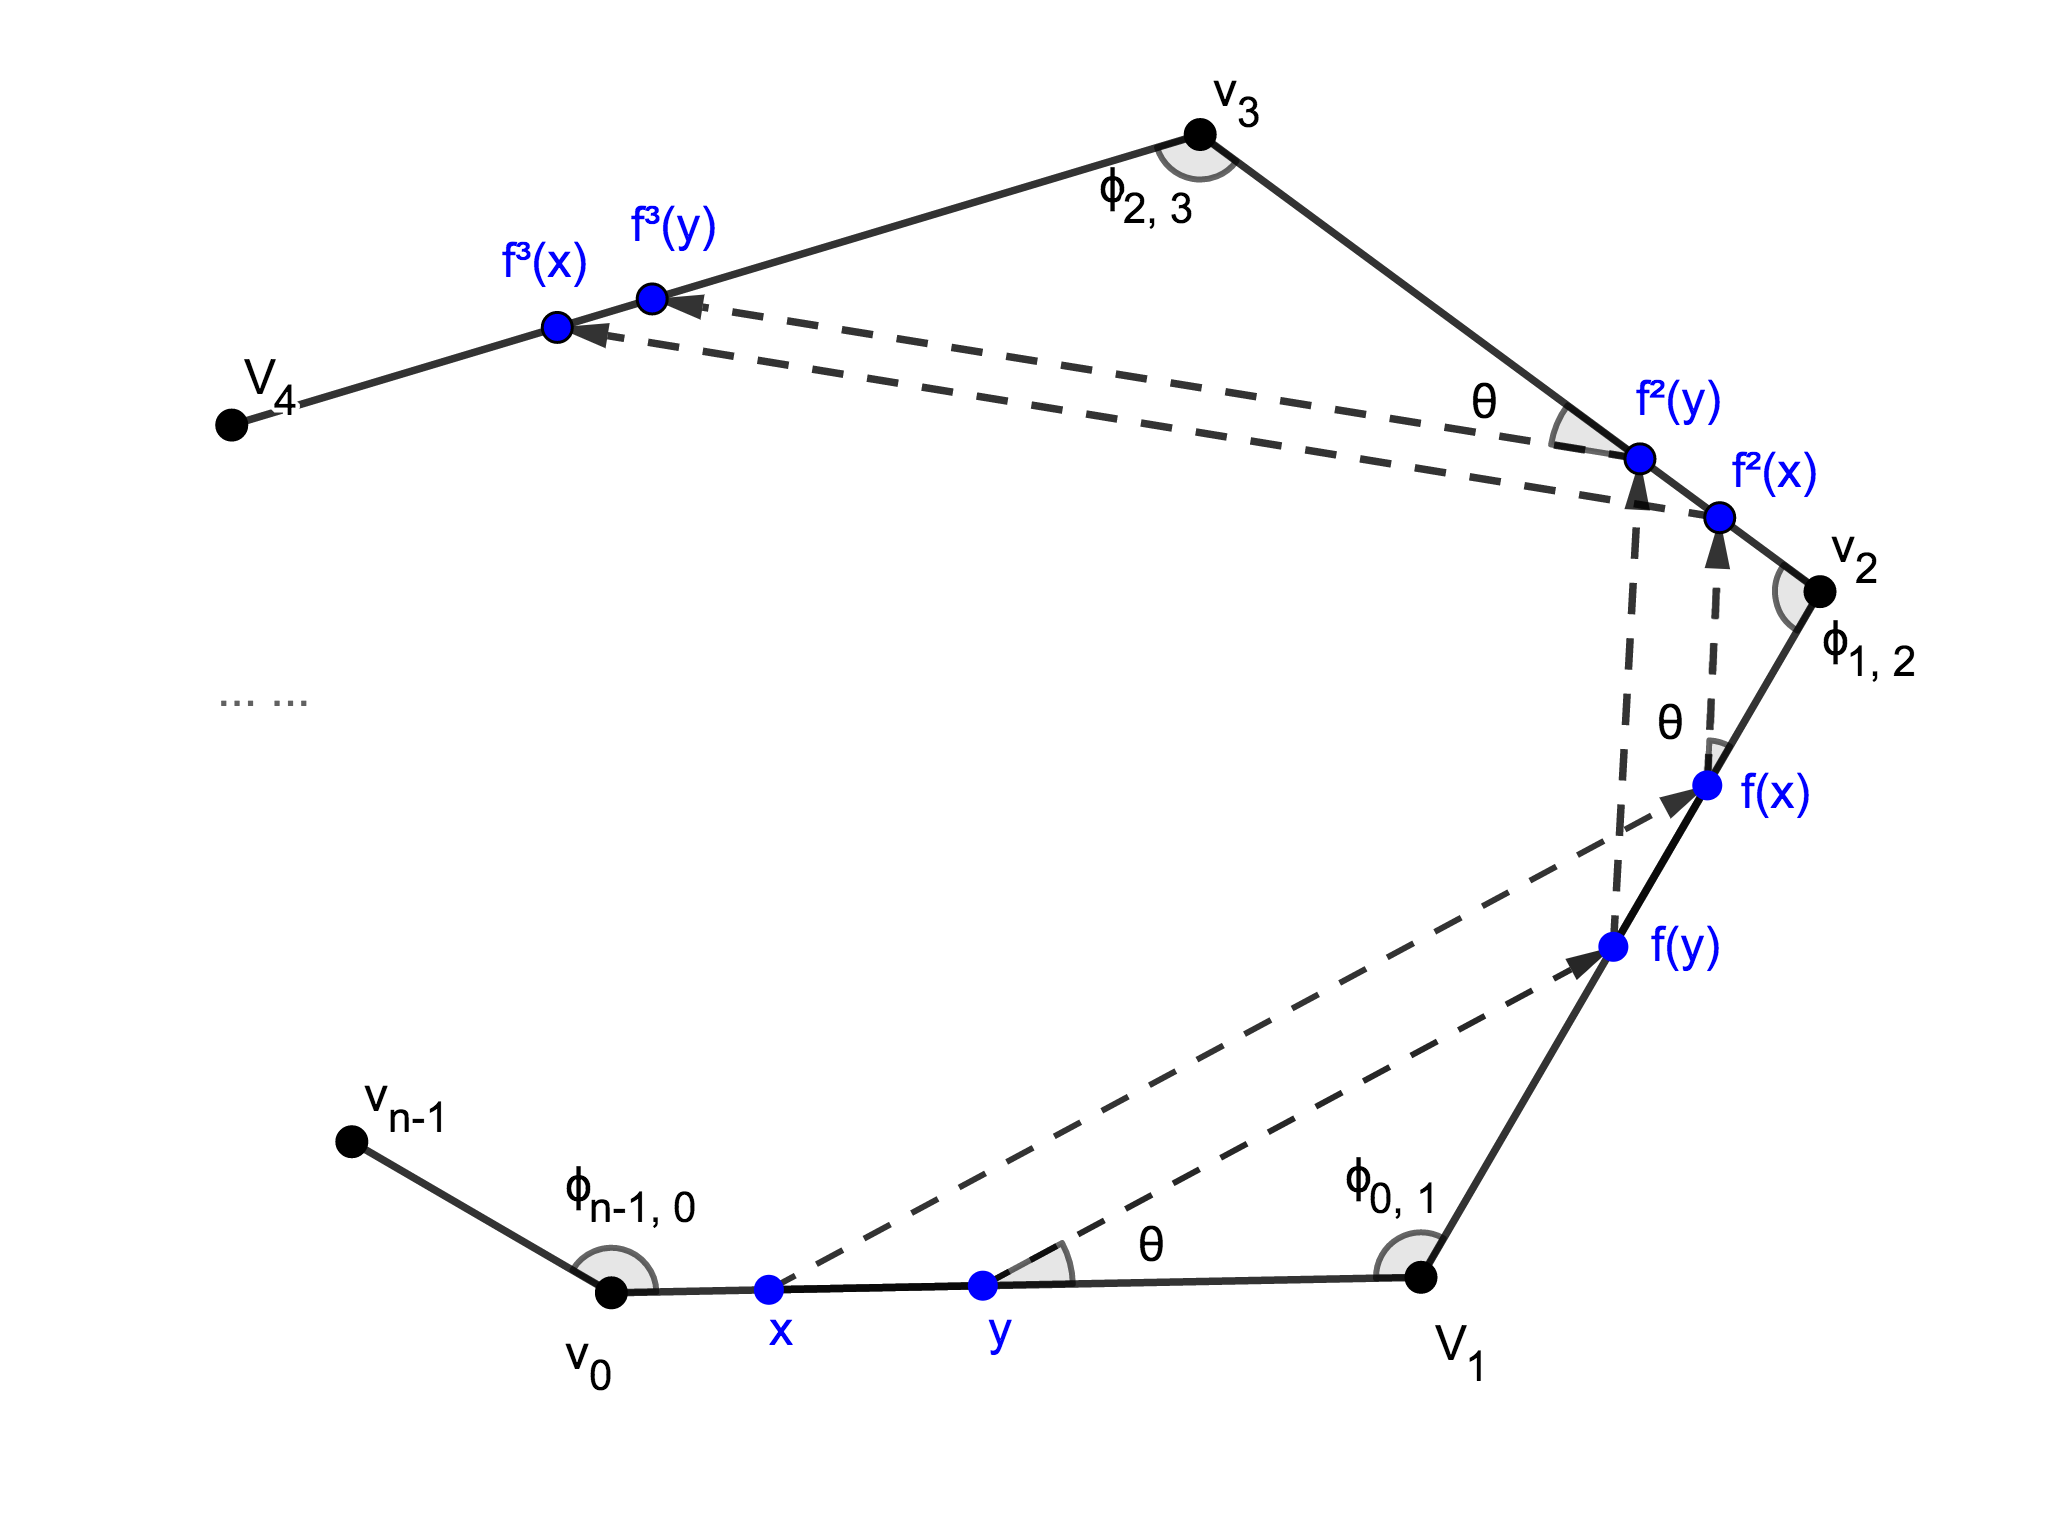
\includegraphics[width=0.6\linewidth]{figures/convex_cycle.png}
    \centering
    \caption{The contracting cycle in a convex polygon.\label{fig:conv_cycle}}
    \centering
\end{figure}
Without loss of generality, assume $\theta \in (0, \frac{\pi}{2}]$. Consider the
triangle formed by two adjacent edges $e_i$, $e_{i+1}$ of $P$. The robot will
bounce from $e_i$ to $e_{i+1}$ regardless of its start position if and only if
$\theta \in (0, \angle v_{i+2}v_{i}v_{i+1})$. Thus, the robot will always bounce
to the next adjacent edge if and only if
$\theta \in (0, \min_{i}(\angle v_{i+2}v_{i}v_{i+1})$.

Suppose we have two start positions $x$ and $y$ on edge $e_0$ and the two
corresponding trajectories under fixed angle $\theta$. Denote the robot's
position on $e_k$ after bouncing $k$ consecutive edges as $f^{k}(x)$ and
$f^{k}(y)$ respectively. $\triangle f^{k}(x)v_{k+1}f^{k+1}(x)$ and
$\triangle f^{k}(y)v_{k+1}f^{k+1}(y)$ are similar triangles since they share a
common internal angle of the polygon, $\pi - \phi_{k,k+1}$, and the bouncing angle
$\theta$.

The distance between the two trajectories on $e_0$ after the robot bounces off
every edge of the polygon, i.e., bounces off $n$ times, is
$d(f^{n}(x), f^{n}(y))$.

Since function composition multiplies the coefficients $C(\theta, \phi)$, 
the distance between $x$ and $y$ changes after one orbit of the polygon by the
ratio

\begin{eqnarray*}
\frac{d(f^{n}(x)), f^{n}(y))}{d(f^{0}(x), f^{0}(y))} = \prod_{i = 0}^{n-1}
C(\theta, \phi_{i-1, i}).
\end{eqnarray*}

If $\prod_{i = 0}^{n-1} C(\theta, \phi_{i}) < 1$, then $f^k(x)$ is a contraction
mapping from $e_0$ back to iteself, and by the Banach fixed-point theorem, it
has a unique fixed point \cite{Granas2003}.

Since all transition in this example are right transitions, the constraint $C(\theta,\phi_{i-1, i})<1$ is equivalent to $\theta < \frac{\pi}{2}-\frac{\phi_{i-1, i}}{2}$. So we can guarantee that this condition holds for the orbit by requiring

\begin{equation*}
\theta \in (0, \min(\min_{i = 0, 1, \dots, n-1}(\angle v_{i+2}v_{i}v_{i+1}),
\frac{\pi}{2}-\frac{\phi_{i-1, i}}{2})),
\end{equation*}

in which case the fixed-angle bouncing strategy with $\theta$ leads to a convex
$n$-cycle regardless of the robot's start position.
\qed

\end{proof}


{\color{red} compelling example to reward people for getting through all this:
robot starts at large interval in convex poly with small doorway, and cycles
until it reduces uncertainty enough to transition}

\begin{figure}
    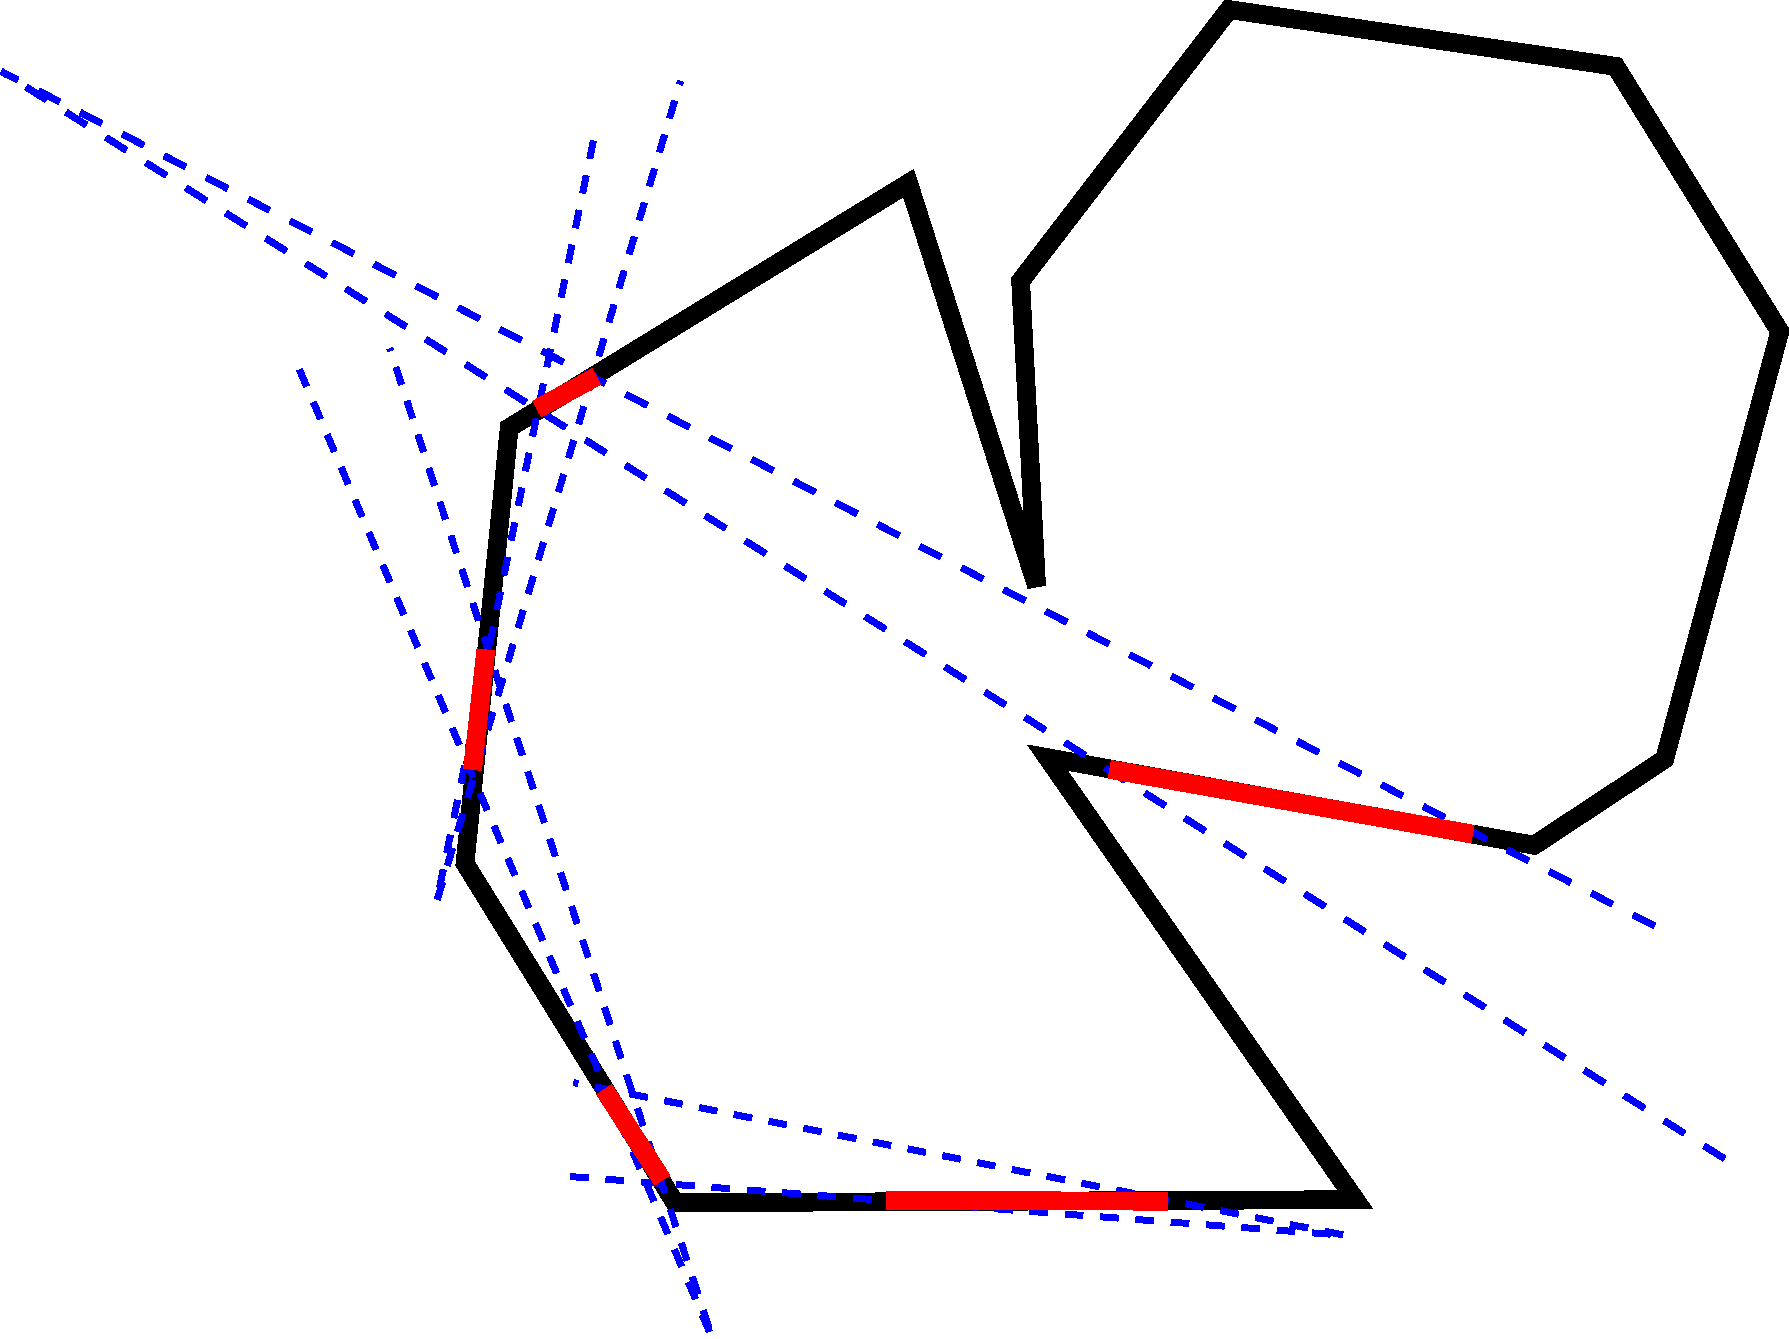
\includegraphics[width=0.6\linewidth]{figures/bounce_preimages.pdf}
    \centering
    \caption{An example of how contraction properties can be used to control
robot state uncertainty enough to navigate the robot through a narrow doorway,
even with a lower bound on angle error. The dotted lines show a 
parameterization of preimages.}
\label{fig:preimage_example}
\end{figure}


\section{Applications}

We have presented data structures (the bounce visibility diagram and bounce
visibility graph, augmented with contraction information) which can be applied
to several different strategy synthesis problems in mobile robotics. Indeed, we
are only scratching the surface of possible applications and extensions.

\subsection{Concise Strategies for Navigation}

Here, we define the \emph{navigation} task. Informally, we wish to decide if
there is a strategy which uses only nondeterministic bounce laws which can cause
the robot to move from any point in a given set of starting points in $\partial P$ to
another given goal set. We require that the start and goal sets are
convex (a single interval $[s_1, s_2] \in \partial P$).


\begin{definition}
\textbf{Navigation}:
Given a polygonal environment $P$, a starting convex set $S \in \partial P$ of possible robot positions along the
environment boundary, and a goal convex set $G \in \partial P$, determine a strategy $\pi$ which
will be guaranteed to take the robot from any point in $S$ to a point in $G$, or
determine that no such strategy exists.
\end{definition}

\subsubsection{Navigation with Safe Actions} \label{sec:safe}

We can create a \emph{safe roadmap} out of the bounce visibility graph by
traversing all edges and removing edges with an empty $\tilde{\theta}_{max}$,
and labelling the remaining edges with the interval of safe actions.

The resulting graph, $G_{safe}$, can be used to generate strategies for the
robot which take it from segment $i_{start}$ to segment $i_{end}$: each path in
$G_{safe}$ from the node corresponding to $i_{start}$ to $i_{end}$ represents
such a strategy.

Moreover, the edge
information along the path can be used to create more concise strategies: to
determine if a path can be executed using a constant controller $b(\alpha,
\theta) = \theta$, intersect all the intervals along the path and check if the
resulting interval is nonempty. If it is, the path may be executed with any
$\theta$ in that interval. In general, deciding whether a given path may be
executed with $k$ constant fixed bounce law controllers is the interval
hitting-set problem, which is NP-hard, though in practice we are mostly
interested in small $k$ {\color{red} more caveats about why this is not so bad}.

Given two or more paths of the same length, we may intersect their angle
constraints at each respective step, and create a strategy which is capable of
executing both paths (or determine that no such strategy exists).

However, navigation with safe actions is not complete. {\color{red} example,
characterization}

%\begin{lemma}
%Given points $x,y \in \partial P$, let $v_x \in V(BVG)$ be the node representing
%the segment in $\Pi$ that contains $x$, and $v_y$ be the node corresponding to
%the segment containing $y$. Then, a path in $BVG$ from $v_x$ to $v_y$ corresponds
%to a family of strategies which take a robot from $x$ to the segment containing
%$y$.
%\end{lemma}
%
%\begin{proof}
%By Lemma \ref{def:transition}, each edge in the path from $v_x$ to $v_y$
%describes a family of bounce laws which can take a robot from any point in the
%source edge to a point in the target edge. The transition functions represented
%by these families can be composed together {\color{red} how exactly to do this
%is not clear}
%\end{proof}


%The crux of the algorithm is that we can determine which transitions between
%edges of $P'$ admit intervals of departure angles $\tilde{\theta}$ under which
%\emph{any} point in $e_i$ can transition to \emph{some} point in $e_j$.
%
%Thus, a path in the bounce visibility graph represents the composition of such guaranteed transitions.

\begin{algorithm}
\caption{Generating a nondeterministic bounce strategy for navigation from any
point in start set $S$ to a point in goal set $G$.}
\label{algo:nav}

\begin{algorithmic}
\Procedure{Navigate}{$poly$, $G$, $S$, $criterion$}
\State $BVD \gets$ \Call{PartitionPoly}{$poly$}
\State $G_{safe} \gets$ \Call{mkSafeGraph}{$BVD$}
\State $paths \gets$ \Call{GetAllPaths}{$BVD$, $G$, $S$,$k$}
\Comment $k$ is an upper bound on the path length
\State $strategy \gets$ \Call{getStrategy}{$paths$}
\EndProcedure
\end{algorithmic}
\end{algorithm}

%For a sequence of transitions $f_1, \ldots, f_k$,

%$\max_{i \in \{1,\ldots, k\}}( \min(angle\_range(f_i) ))$

%
%We would like to chain together nondeterministic transitions such that each
%transition is guaranteed to land in the "basin" of the next.

%We use pre-image backchaining to determine sequences of edges which might allow
%such transitions, based on visibility properties. This is found through a simple
%breadth-first search through the graph from the goal to the start.

%Then, we must determine strategies which can execute these series of transitions
%from the start interval. This is done using forward projection from the start
%set.

%It is possible that paths without loops may be impossible without
%more precise knowledge of the robot's position than is available (see Case 2 in
%Proposition 2).
%
%There are several methods of dealing with this. We can reduce uncertainty by
%finding a nearby limit cycle and including it in our path, allowing us to
%arbitrarily reduce uncertainty. We can use
%contraction mappings along the way to reduce uncertainty in a similar way.

\subsection{Backprojections for Navigation}

We have three degrees of freedom when computing action preimages - the angle
interval and the size/location of the subinterval.

There are two natural quantities we may wish to maximize for such a transition -
the size of the subinterval, or the size of the angle interval.
The maximum angle interval will always be a point. Imagine an interval on $i$
which allowed for a maximal angle range $[\theta_{min}, \theta_{max}]$ that
guaranteed a transition from any point in the interval to $j$. By
shrinking this interval to a point, we must increase the size of the angle
interval, creating a contradiction. The maximum size subinterval will always correspond to a singleton angle range,
$\theta$, such that $l_{sub}$ and $r_{sub}$ are parallel. The location of this
interval will depend on the local geometry.

Case 1: start set is entirely contained within equivalence class

Case 2: start set is split across equivalence classes (make strategies for
subsets of start set and intersect - what kinds of strategy intersections make
sense?)

could be multiple paths with same number of bounces that get to goal set

reachability vs. guaranteed-along-all-paths


%\subsubsection{Constant Fixed Angle Controllers}
%
%If we wish to treat the special case of a constant controller $b(\alpha, \theta)
%= \theta$, we could find a strategy as described in Algorithm \ref{algo:nav} and
%then inspect the strategy to see if it admits a constant controller. However,
%this approach is not complete, since a different bounce sequence may allow a
%constant control strategy while than the one found by preimage backchaining.
%
%For a complete (up to bounded length) algorithm, we may incorporate the
%constraint on constant $\theta$ into the search procedure. At each step in the
%backwards search from the goal set, maintain an interval of angles which allow
%all the previously found transitions.

\subsection{Relative Bounce Law Analysis}

given initial position and orientation, can generate new visibility graph for
all possible relative angles.


\subsection{Patrolling}

We define the \emph{patrolling} task as:

\begin{quotation}
Given an environment $P$, a set of possible starting states $S$, and
a sequence of edges of the environment $E = \{e_1, \ldots, e_k\}$,
determine a strategy which causes the robot to visit each edge of the sequence
in order on a repeatable path.
\end{quotation}

This task is related to the Aquarium Keeper's Problem in computational
geometry \cite{czyzowicz1991aquarium}.

And a weaker task:

\begin{quotation}
Given an environment $P$, a set of possible starting states $S$, find a limit
cycle reachable from all points in $S$ under the same strategy.
\end{quotation}


\begin{definition}
A sequence of transitions $f_1 \circ \ldots \circ f_k$ is \textbf{strongly
contracting} if $\forall i \in \{1, \ldots, k\}, f_i$ is a contraction mapping.
\end{definition}

\begin{corollary}
Every polygon will produce a bounce visibility graph containing at least two
strongly contracting cycles, for $\theta \in [0, \phi_{min}/2]$ and $\theta \in
[\pi - \phi_{min}/2, \pi]$.
\end{corollary}

\begin{proof}

Let the robot have a constant fixed angle bounce strategy, so it always leaves
the boundary at angle $\theta \in [0,\phi_{min}/2]$ counterclockwise from the
boundary.

At each transition, the robot will either strike the next adjacent edge in
$P$, or a reflex vertex will cause the robot to strike some other edge in the
polygon. Either way, the transition is guaranteed to be a contraction mapping by
the definition of $\phi_{min}$ and Lemma \ref{lemma:angrange}.

Eventually, this strategy will produce a strongly contracting cycle. Each
transition moves the robot from one edge to another, so at some point, the
robot's trajectory must return to an edge it has previously visited. The series
of transitions in this trajectory corresponds exactly to a strongly contracting
cycle in the bounce visibility graph.
\qed

\end{proof}

Note that the previous proof does not guarantee a limit cycle in every polygon.
It is possible to construct polygons such that the locations of the collision
points in the stable limit cycle do not all fall within the edges forming the
strongly contracting cycle. However, the only examples of such that we have been
able to construct are in general position and are unlikely to occur in practical
applications.

\begin{lemma}
cycles can contain non-contracting bounces - there are lots of cycles
\end{lemma}

Algorithm: finding limit cycles is done by finding cycles in graph with
contraction coefficient less than 1

\subsection{Localization}

\begin{definition}
A localization strategy is a nondeterministic strategy that produces paths all
ending at the same node, from a starting set.
\end{definition}

Connect to Shell/Alam/Bobadilla work on limit cycles for localization.

\subsection{Comparing Bounce Laws}

\begin{theorem}
reachability of graph gives ordering on the power of bounce laws
\end{theorem}


\section{Open Questions and Future Work}



{\color{red} 
\begin{itemize}
\item efficient synthesis for navigation and localization - optimization formulation?
\item characterization of swaths of bounce laws
\item ergodicity / chaotic trajectories
{\color{red} add todd murphey ergodic paths, and that other ergodic path one steve
found, and the chaotic controller papers}
\end{itemize}
}

We are very interested in using the dynamical properties of this robot model to
create controllers which produce ergodic motion, where the time-averaged
behavior of the system approaches the space-averaged behavior, causing the robot
to not spend ``too much" time in any given part of the state space. Measures
of ergodicity have recently been used in exploration tasks
\cite{miller2016ergodic}. Chaotic dynamical systems have also been used directly
as controllers for mobile robots \cite{nakamura2001chaotic}.

\begin{corollary} bounce angle range returned is correct, and optimal
   (largest range)
\end{corollary}


%\subsubsection{Incorporating other Sensor Models}
%
%\section{Examples}
%
%\subsection{office space w/ long hallway}
%\subsection{``almost symmetric" environment}
%\subsection{worst case complexity}
%
\iffalse

{\small
\begin{center}
\begin{quotation}
``Geometry is not true, it is advantageous." \\
\hfill    --- Henri Poincar\'e
\end{quotation}
\end{center}
}


%%%%%%%%%%%%%%%%%%%%%%%%%%%%%%%%%%%%%%%%%
\section{Introduction} 

This control strategy is largely chosen because of the ease of implementation.
It requires much less fine-grained proprioception than many other mobile robot
control algorithms, needing the robot to only have the ability to move forward
until reaching some obstacle, then the ability to rotate in place. We assume
from the beginning that there will be nondeterministic error in both of these
operations - especially when wheels are independently powered, robots rarely
move forward in truly straight lines, and rotation-in-place is similarly
difficult to achieve precisely. Both of these types of error are accounted for
by our nondeterministic state propagation. In fact, our approach does not assume
a fixed error distribution or range, but in fact produces the maximum allowable
error values constructively. Thus, this work lends itself well to the mobile
robot system design process - users can iteratively design environments and
robots such that the desired task has a strong guarantee of success.

The only type of error we do not
account for is ``sliding" along the environment boundaries, which may occur
during rotation or collision. However, many common commercial mobile robots
(such as vacuum robots) do not experience appreciable sliding.

% There has been rising interests in minimum sensing robots in recent years as swarm robots become more and more popular. 
In this paper, we consider simple robots with "bouncing" behaviors: robots which
travel in straight lines in the plane, until encountering an environment
boundary, at which point they rotate in place and set off again. A growing line
of work is considering the computational power of individual bouncing strategies
and their applications to robotic tasks and applications in biological contexts
\cite{ErLav13}, \cite{microorganism2017}, \cite{alam2017minimalist}.

We introduce a combinatorial, visibility-based data structure to organize and
compare these bouncing strategies in simple polygonal environments. The overall
idea is to discretize the environment boundary using visibility information,
creating equivalence classes (segments along the boundary) where the robot has a
similar set of choices from any point in the segment. We then construct a graph
representation of this environment where nodes are segments of the boundary, and
edges are transitions between segments (with associated control strategies). We
then extend previous results on the dynamics of composed transitions
\cite{NilBecLav17}, which give convenient guarantees on the stability of cycles
and contraction of robot state uncertainty. Finally, we demonstrate how to
formulate many common mobile robotic tasks as queries to this data structure.


\subsection{Robot Motion Model}\label{subsec:bounce_strategy}

A polygon is in general position if no $3$ vertices lie on the same line. For
the rest of this paper, we assume all polygons are in general position. All
index arithmetic is $\mod n$ throughout the paper.

A \textbf{bouncing strategy} describes the robot's configuration change when it
encounters the boundary of a polygon. We will only consider the bounce occurred
inside an open edge of the polygon: the robot's behavior is undefined at a
vertex of the polygon.

A bouncing strategy defines a function space, where each function maps between 
points of the environment boundary, parameterized by the incoming trajectory
angle and optionally an angle $\theta$.

%Each bouncing strategy has a characterization function
%for $\vec{m}$ over parameters $\vec{n}$ and $\vec{l}$, where $\vec{n}$ is the
%unit vector for the normal of the bounce-off wall, $\vec{l}$ is the unit vector
%for the incoming direction, and $\vec{m}$ is the unit vector for the outgoing
%direction.
%
%\begin{itemize}
%    \item Specular Bounce (Billiard): $\vec{m} = f(\vec{l}, \vec{n})$, where \begin{eqnarray*}
%    f(\vec{l}, \vec{n}) = \vec{l} - 2(\vec{l}\cdot \vec{n})\vec{n}
%    \end{eqnarray*}
%    (``$\cdot$'' is the dot product operation between two vectors), which is equivalent to $(\vec{l}+\vec{m}) \cdot \vec{n} = 0$. This bouncing behavior is elastic and follows the most natural law: the incoming angle equals the outgoing angle \cite{geometry_billards}.
%    \item Fixed Angle Bounce: $\vec{m} = f(\vec{n}, \theta)$, where $\theta$ is a constant in $[-\frac{\pi}{2}, \frac{\pi}{2}]$, and \begin{eqnarray*}f(\vec{n}, \theta) = 
%    \begin{bmatrix} 
%    \cos(\theta) & \sin(\theta)\\
%    -\sin(\theta) & \cos(\theta)\\
%    \end{bmatrix}\vec{n}.\end{eqnarray*} In other words, the robot always bounces off the wall at a fix angle with respect to the normal.
%    \item Monotonic Fixed Angle Bounce: $\vec{m} = f(\vec{l}, \vec{n}, \theta)$, where $\theta$ is a constant in $(0, \frac{\pi}{2})$. Let $s = det(\begin{bmatrix} 
%    \vec{l}.x & \vec{l}.y\\
%    \vec{n}.x & \vec{n}.y\\
%    \end{bmatrix})$, and $\theta' = \frac{s}{|s|}\theta$ ($|s|$ denote the absolute value of $s$; the behavior for $|s| = 0$ is undefined). Then \begin{eqnarray*}f(\vec{l}, \vec{n}, \theta) = 
%    \begin{bmatrix} 
%    \cos(\theta') & \sin(\theta')\\
%    -\sin(\theta') & \cos(\theta')\\
%    \end{bmatrix}\vec{n}.\end{eqnarray*} This bouncing strategy is very similar to the Fixed Angle Bounce except for the monotonic restriction that the robot's incoming path and outgoing path have to be on the opposite sides of the normal.
%    
%    \item Relative Angle Bounce: $\vec{m} = f(\vec{l}, \beta)$, where $\beta$ is a constant in $[0, 2\pi)$, and \begin{eqnarray*}f(\vec{l}, \beta) = \begin{bmatrix}
%    \cos(\beta) & -\sin(\beta)\\
%    \sin(\beta) & \cos(\beta)\\
%    \end{bmatrix}\vec{l}.
%    \end{eqnarray*} The robot will rotate a fixed angle $\beta$ counter-clockwise when encountering the wall. It is possible that this rotation will cause the heading of the robot to still be facing into the wall, in which case this model usually has the robot perform the rotation again until it's heading points into the free space.
%\end{itemize}

% fixed vs. monotonic fixed vs. relative vs. specular

% parameterization for monotonic bounces: alpha + beta + gamma = pi

% all bounces are some function of incoming angle and wall normal


\subsection{Link diagram}

The link distance between two vertices in a polygon is the minimum number of line segments inside the polygon connecting the two vertices. The link distance between visible vertices is $1$. In Fig~\ref{fig:link_dis}, the link distance between $v_1$ and $v_2$ is 3.

The link diagram, as introduced in \cite{tan_sweep}, displays the link distance between any two points on the boundary of the polygon. The link diagram is our main motivation for creating a visibility diagram augmented with bouncing information.
\begin{figure}
    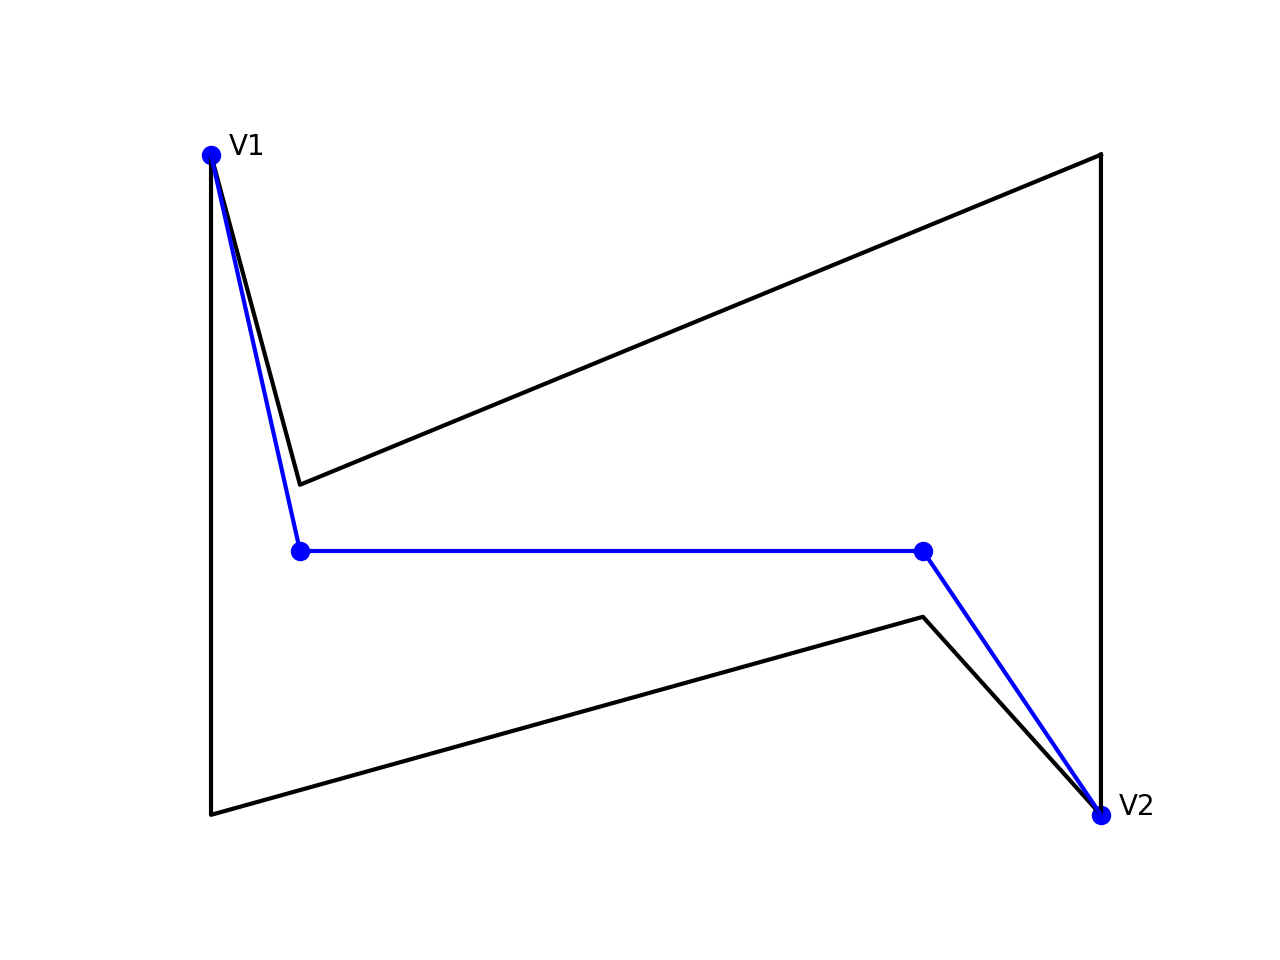
\includegraphics[width=0.6\linewidth]{figures/link_distance.png}
    \centering
    \caption{The link distance between $v_1$ and $v_2$ is 3, as shown by the three blue line segments connecting the two vertices.}\label{fig:link_dis}
    \centering
\end{figure}

\section{Bounce Visibility Diagram \label{bvd_def}}
We will now define the central structure for this paper, the
\textit{Bounce Visibility Diagram} for polygon $P$. We will first insert all new
vertices from the partial local sequence for all vertices into the
polygon $P$, creating the new polygon $P'$ with $m$ vertices. Each of these new
vertices marks a combinatorial change in the visibility polygon at the boundary
of the polygon as an agent traverses the boundary.

The $x-$axis of the diagram parameterizes the boundary of the new polygon,
denoted as $\partial P'$, in counterclockwise order as the interval $[0, m+1)$. The
enpoints of this interval are identified, though for visualization purposes we
do not represent this explicitly. We map every
point in $\partial P'$ to a point in $[0, m+1)$; vertex $v_i$ on $\partial P'$
will map to $x = i$; all points in the open edge $v_iv_{i+1}$ will uniformly map
to $(i, i+1)$. Let $f: [0, m+1)\mapsto \partial P'$ denote this
parameterization. We will generally use the variable $s$ to refer to points on
the boundary of $\partial P'$.

The vertical axis $\theta$ of the diagram has range $[0, \pi]$, representing all
the possible departure angles of the robot from point $s \in \partial P'$. 
At angle $0$, the robot is performing ``wall following": a bounce
to the next counterclockwise vertex.
Let the robot's ``forward direction'' be the direction of the edge that the
robot is on in counterclockwise order.

For each vertex $v_i$, we can define a function $B_i: [0, n) \mapsto [0, \pi]$
for the angle between the robot's forward direction and its direction to vertex
$v_i$ when the robot stands at $f(x)\in \partial P'$. $B_i$ are piecewise
continuous functions; the discontinuities occur when $x$ is an integer, or, in
other words, at the vertices of $\partial P'$. The original vertices in $P$ mark
discontinuities because the angle reference frame for the robot changes when it
moves to a new edge; the new vertices in $P'$ mark discontinuities because the
robot has different vertex visibility view around those vertices, which
motivates us to compute the partial local sequences in the first place.
Fig \ref{fig:bvd} shows an example of the bounce visibility diagram.

%\begin{figure}
%
%\centering
%\begin{subfigure}{0.25\textwidth}
%\centering
%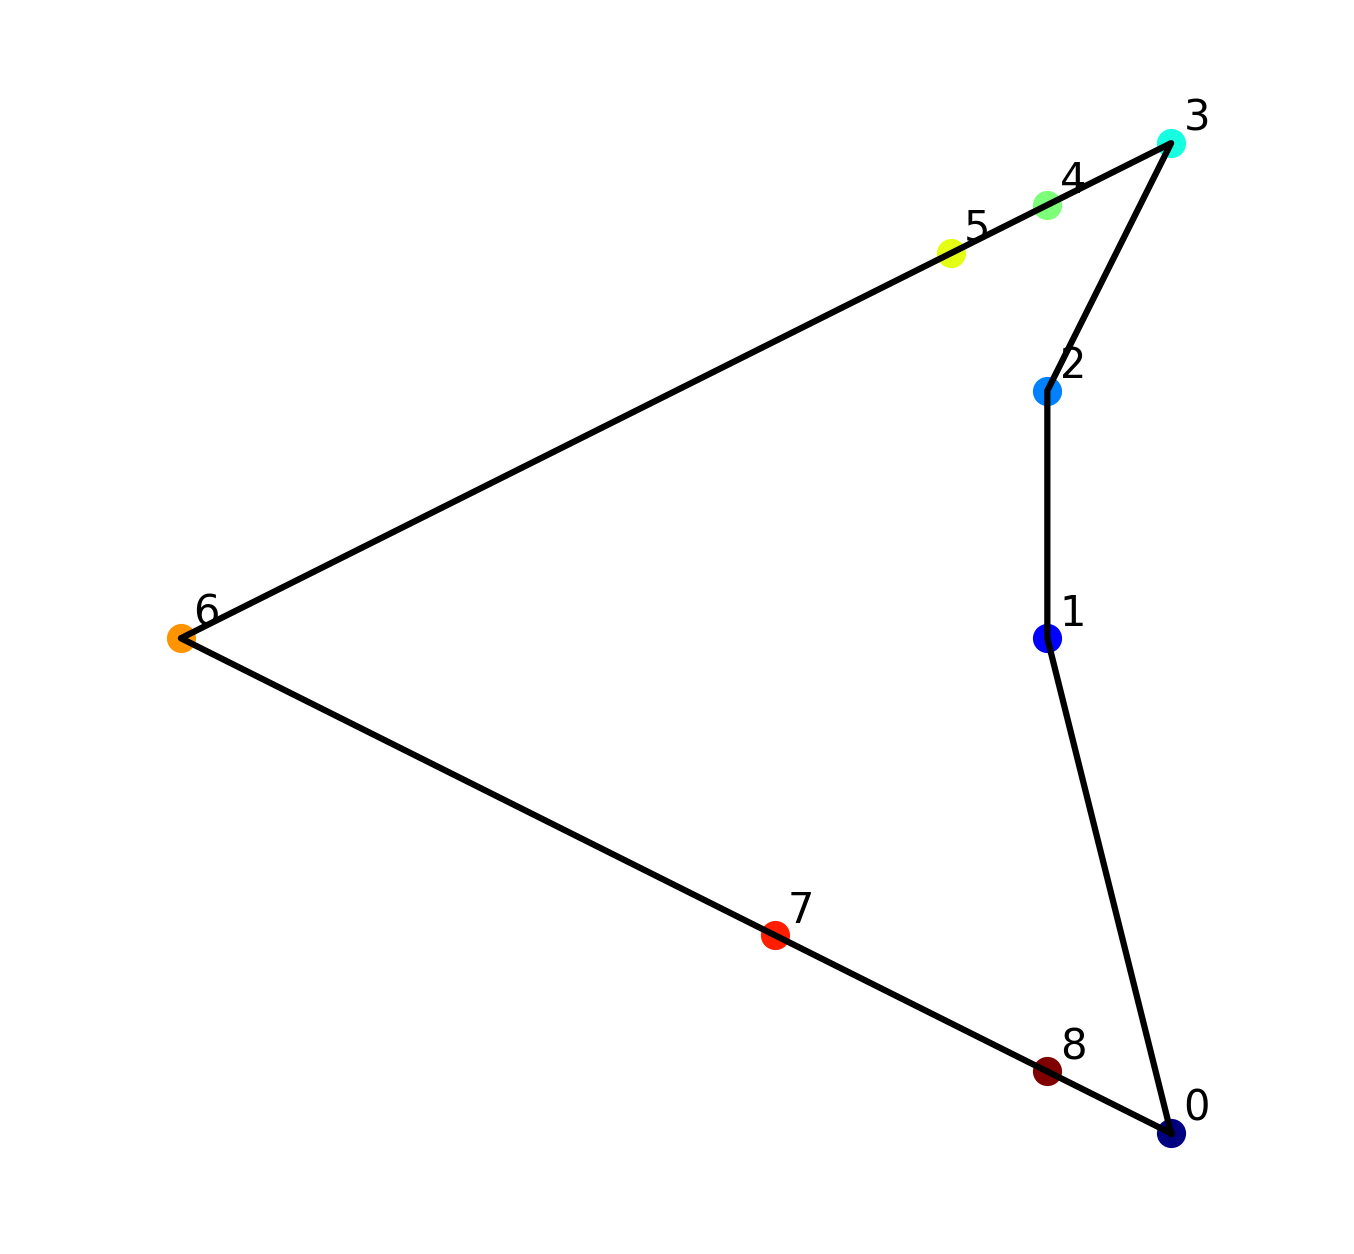
\includegraphics[width=0.7\linewidth]{figures/color_pent.png}
%\captionof{figure}{\label{fig:color_pent}}
%\end{subfigure}%
%\begin{subfigure}{0.25\textwidth}
%\centering
%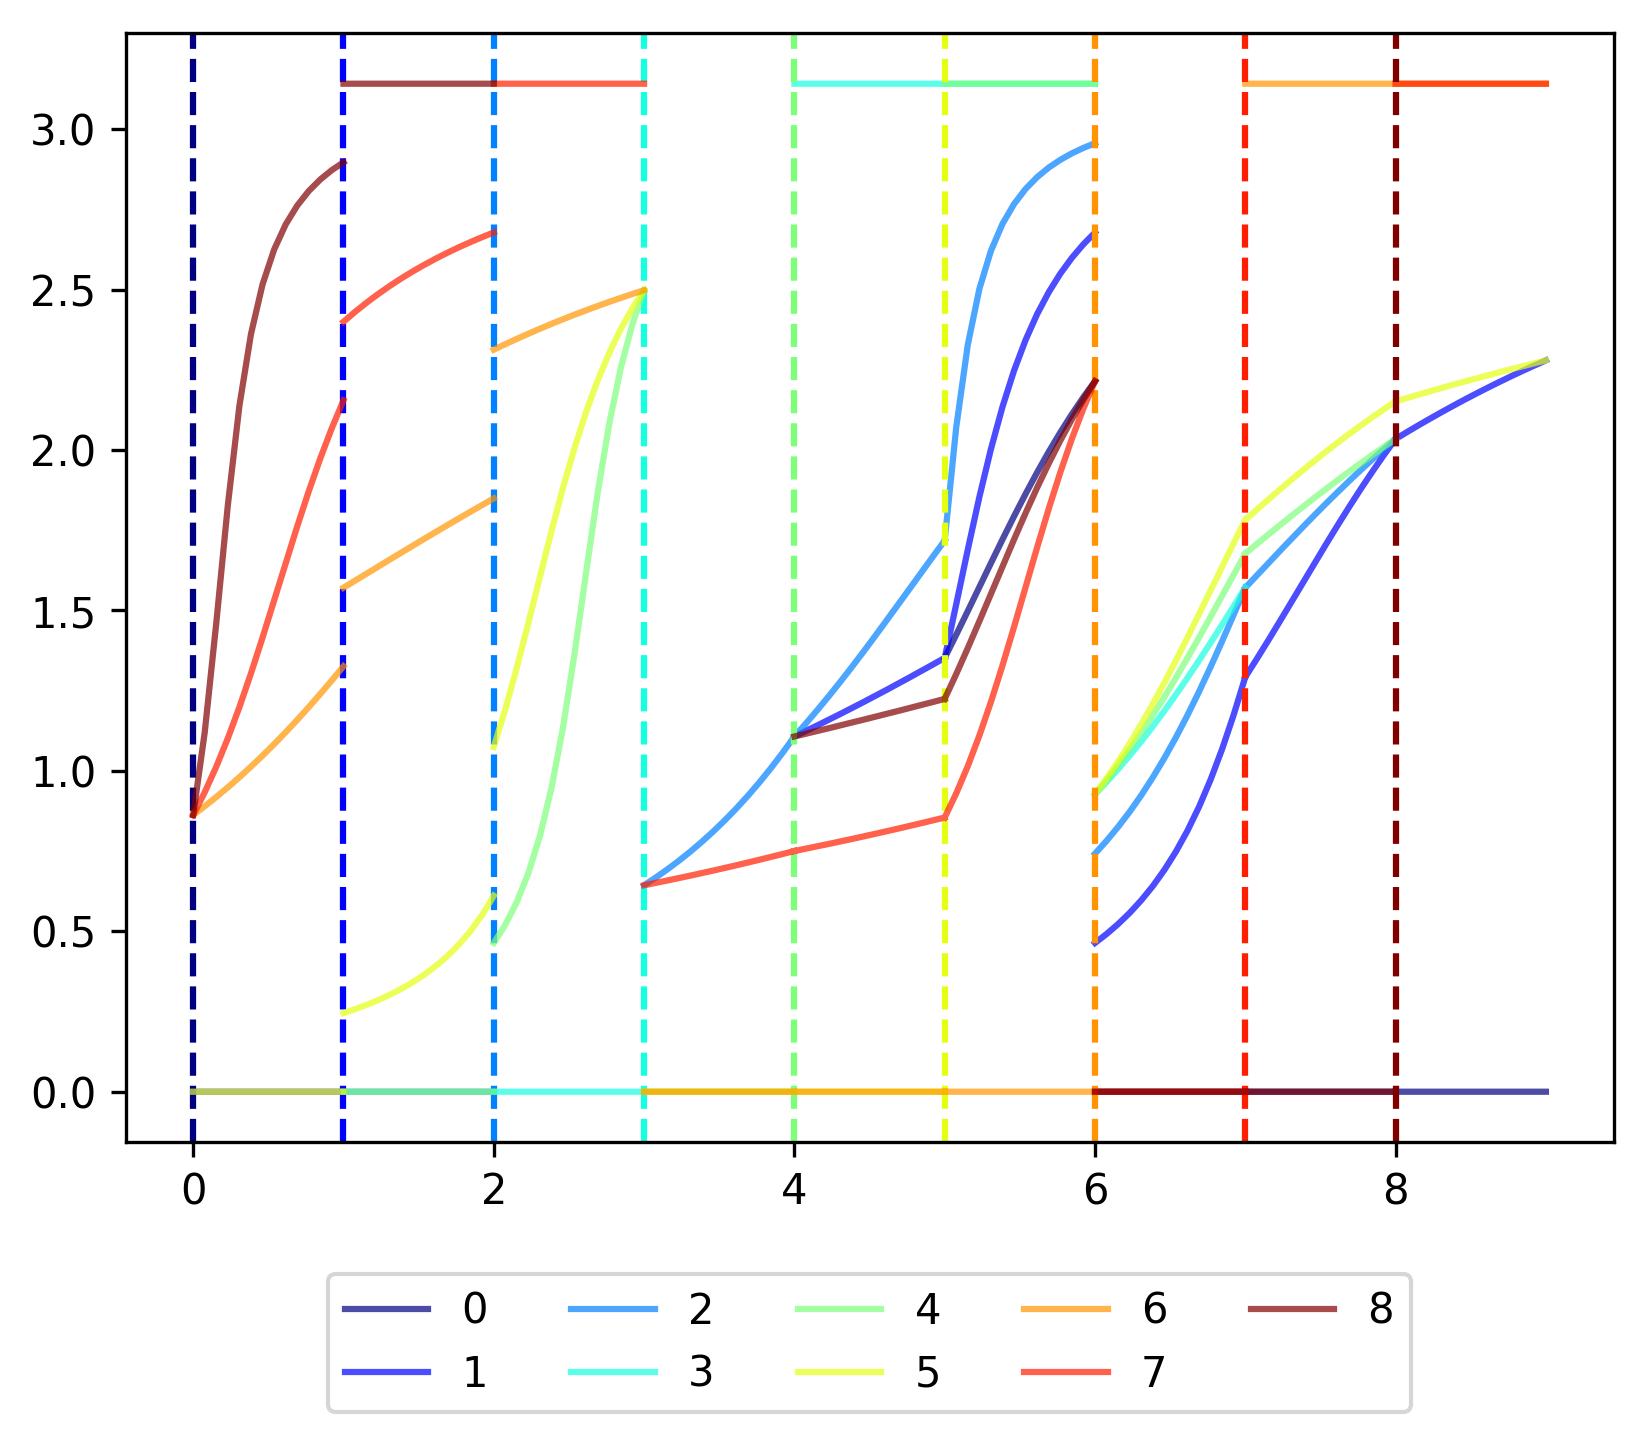
\includegraphics[width=0.8\linewidth]{figures/bvd.png}
%\end{subfigure}
%\caption{A polygon and its corresponding bounce visibility diagram.}
%\label{fig:bvd}
%\end{figure}



\section{BVD as an Information Space \label{bvd_info}}

Information spaces \cite{tovar2005information} are a useful formalism for
reasoning about the information available to a robot as a result of its sensor
and action history. From the \emph{history information space} (the space of all
sensor/action histories), we can define mappings to other, more useful spaces.

Here we will show that the bounce visibility diagram can induce a useful
information space for many mobile robot tasks, and can be augmented with
information from the geometric properties of actuators and sensors.

We will construct $G_{BVD}$, a graph where nodes are segments in the decomposed
environment $P'$ constructed in Section \ref{bvd_def}.

We then define edges in this graph to be transitions between these segments, based on the bounce laws and
required to transition between them. First, we observe that any two segments in
$P'$ that are visible at all are visible along their entire lengths. Thus, we
there exists a function $f$ which maps a point $s \in v_i
v_{i+1}$ to a point $f(s) \in v_j v_{j+1}$ under a bounce at angle $\theta$ from
the normal on edge $v_i v_{i+1}$, for all valid ranges of $s$, $f(s)$, and
$\theta$.

Rather than use $f$ directly, we take a nondeterministic approach and define a
directed transition between edges $v_i v_{i+1}$ and $v_j v_{j+1}$ if it is
possible to reach edge $v_j v_{j+1}$ from edge $v_i v_{i+1}$ under any bounce.
We label the edge with the range of bounce angles, $\theta_{min} < \theta <
\theta_{max}$, under which this is possible. See Figure \ref{fig:bounce_range} for
the geometric definitions of $\theta_{max}$ and $\theta_{min}$.

\begin{figure}
    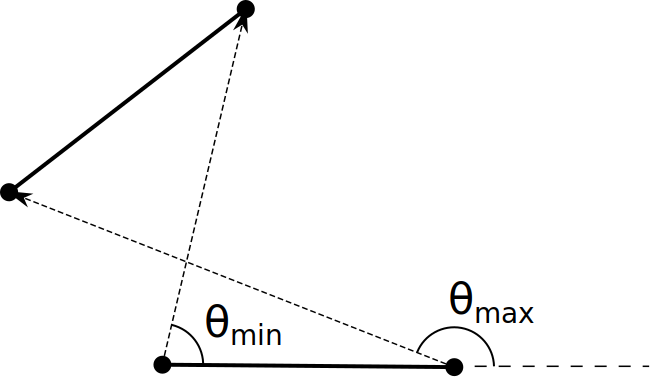
\includegraphics[width=0.8\linewidth]{figures/bouncerange.png}
    \centering
    \caption{Definitions of $\theta_{max}$ and $\theta_{min}$. Can be computed
by rotating the source edge to the x axis without loss of generality.}\label{fig:bounce_range}
    \centering
\end{figure}

\subsection{Augmenting the Graph with Dynamical Information}

We can also add information to the edges in $G_{BVD}$ indicating whether the
mapping from one edge to another is a \emph{contraction mapping}: a transition
which will bring two separate points in the domain closer together in the range,
a useful property for reducing state uncertainty and engineering limit cycles,
as will be discussed in Section \ref{patrol}.

The necessary condition for $f$ to be a contraction mapping is:

\begin{equation*}
|f(x) - f(y)| \leq c |x-y|
\end{equation*}

such that $0 \leq c < 1$.

From Figure \ref{fig:cont_map}, we can see that

\begin{equation*}
|f(x) - f(y)| = \frac{\sin(\theta - \phi)}{\sin(\pi-\theta)} |x-y|
\end{equation*}

from the law of sines, where $\phi$ is the angle between the two edges if they
are extended to their intersection point. If the edges are parallel, a
contraction map is not possible (points will maintain their distance, not shrink
closer together). Thus, whenever $\frac{\sin(\theta - \phi)}{\sin(\pi-\theta)}
< 1$, $f$ is a contraction map, and the edge from $v_i v_{i+1}$ to $v_j
v_{j+1}$ can be labelled as such, with the range of $\theta$ which makes this
condition true.

Furthermore, the contraction property of a composition of multiple bounces can
be determined by simply multiplying the coefficients $\frac{\sin(\theta_i -
\phi_i)}{\sin(\pi-\theta_i)}$, and the constraints on the satisfying angles
$\theta_i$ can be propagated through the composition.

\begin{figure}
    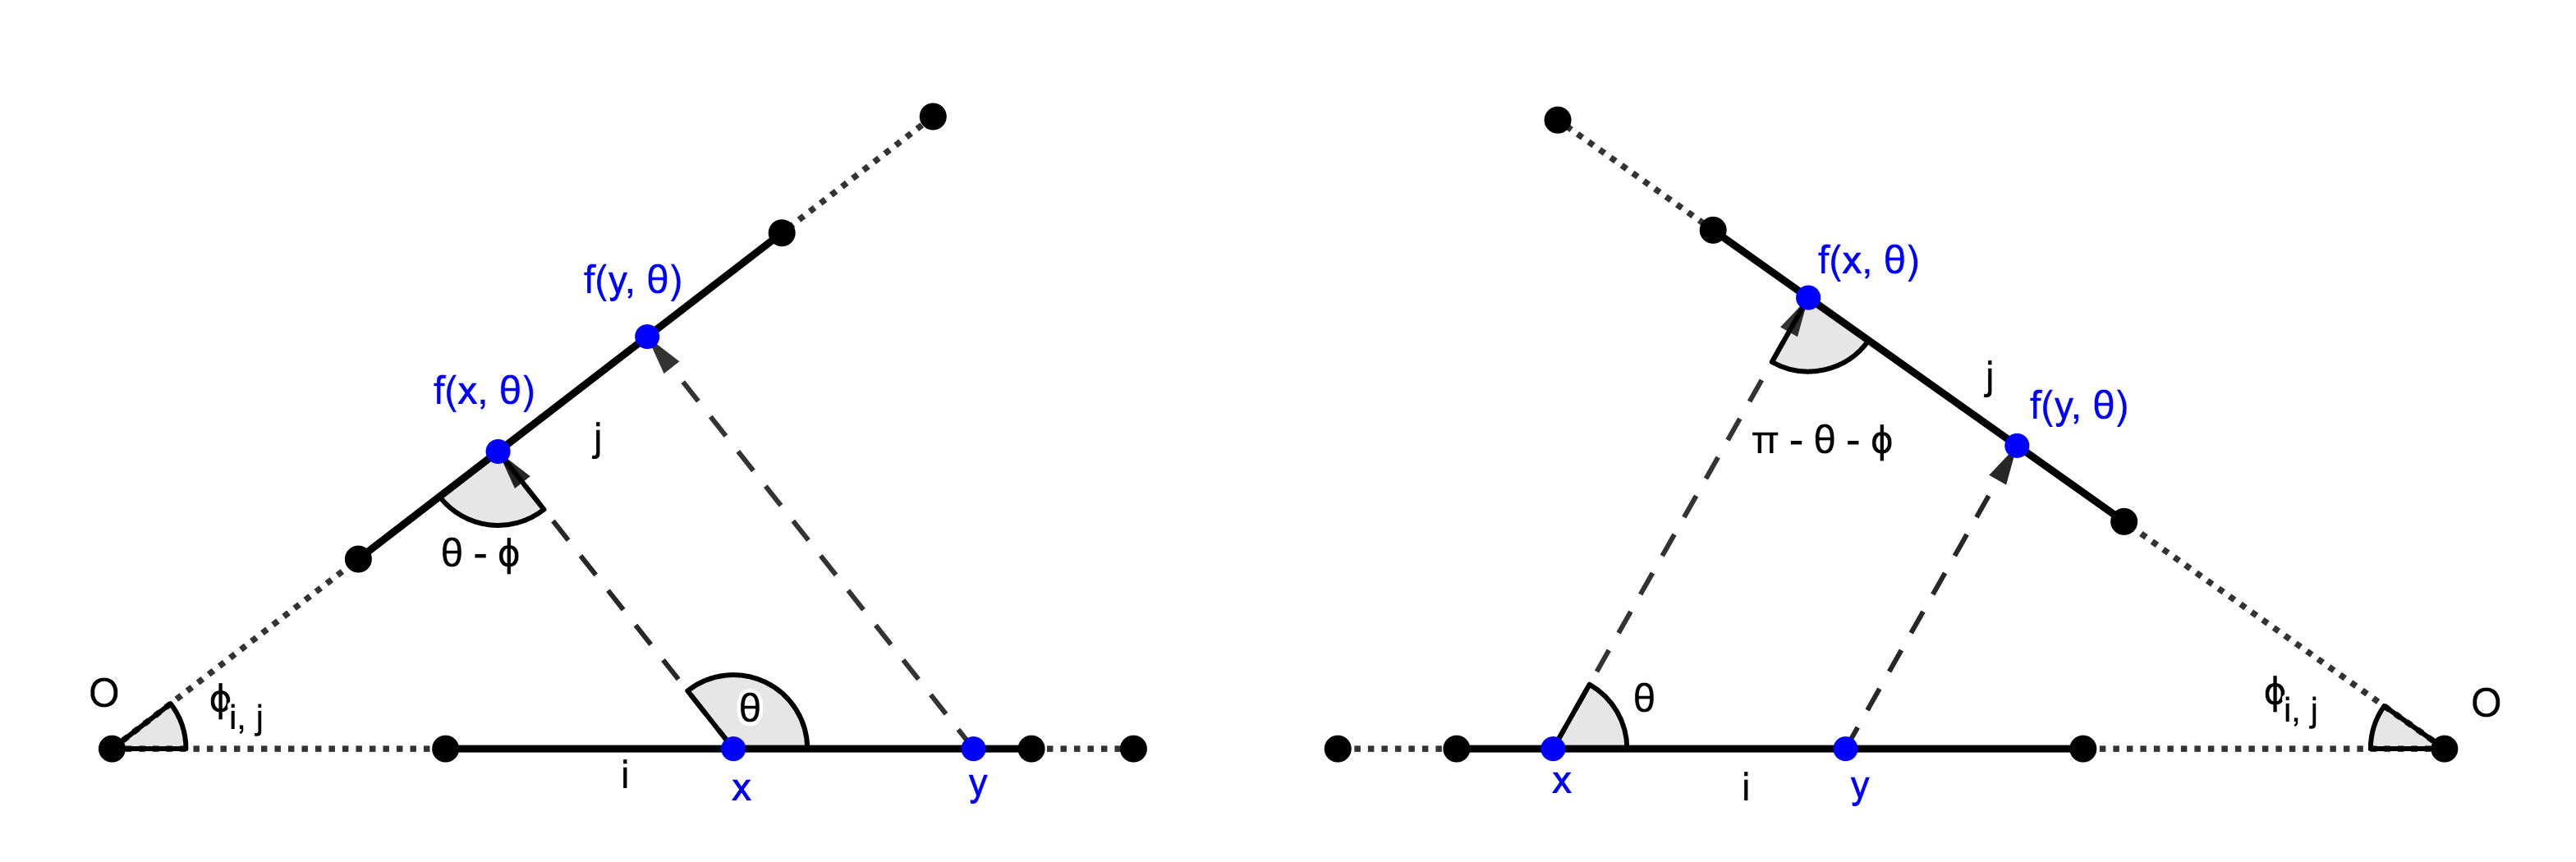
\includegraphics[width=0.8\linewidth]{figures/contraction_map_cond.png}
    \centering
    \caption{\label{fig:cont_map}}
\end{figure}

\subsection{Sensor Modelling}

Here we sketch how different virtual sensors may be incorporated into this
information space representation.

\begin{itemize}
\item \emph{Laser Beams:} laser beams form new, internal edges of the polygon. They can be
added to the bounce visibility graph by marking all the edges which represent
bounces that would cross the laser beam with a special symbol. different symbols
for distinguishable beams. If a beam is encountered, and we are tracking state
as a set of possible segments along the boundary of $P'$, we can reduce
uncertainty in our estimate by only propagating the state estimate
forward along edges with that symbol. To engineer reduction in uncertainty,
we may be able to put laser beams in positions that break graph symmetry.
\item \emph{Pebbles:} pebbles are quite important in many robotic tasks, such as
when we need to guarantee that a wall-following strategy has successfully
circumnavigated a polygon. In this representation, we can simply augment nodes
in $G_{BVE}$ if our robot has placed a pebble in that segment (or we may mark
multiple nodes, then use actions to reduce uncertainty in our state estimate
once we return to the pebble).
\item \emph{Cameras:} Especially when discussing coverage, it is helpful to have
some sense of how we "cover" a polygon's interior. One abstract sensor with this
behavior is a model of a camera, which may have some given range and field of
view. The set-theoretic representation of this visibility region can be used to
represent how much of the polygon may be covered by a given trajectory. Ideally,
coverage strategies would allow for satisfying coverage given nondeterminism in
the start states and actions.
\end{itemize}

\section{Task Formulation}

We will now show how to formulate many common robot task specifications in terms
of the data structure described above. The discretization of the continuous
environment allows us to now reason over trajectories through a graph.




\subsection{Patrolling \label{patrol}}

We define the \emph{patrolling} task as:

\begin{quotation}
Given an environment $P$, a set of possible starting states $S$, and
a sequence of edges of the environment $E = \{e_1, \ldots, e_k\}$,
determine a strategy which causes the robot to visit each edge of the sequence
in order on a repeatable path.
\end{quotation}

This task is related to the Aquarium Keeper's Problem in computational
geometry \cite{czyzowicz1991aquarium}.

In prior work \cite{NilBecLav17}, it was shown that stable limit cycles
exist for constant-angle fixed bouncing in regular polygons, for some ranges of bounce angles.
These results also hold for convex polygons in general.

The general flavor of these results are that the bounce functions from edge to
edge are composed into one function which returns the robot to its starting
edge. If this function is a contraction map, a fixed point exists on the
starting edge, and thus a limit cycle of the robot's trajectory exists. The
exact conditions of the existence of this limit cycle depend on the product of
the contraction coefficients being less than one; and on $\theta$ being such
that the bounce at each stage can actually occur. All of the information
necessary to check these conditions is in $G_{BVD}$, as described in Section
\ref{bvd_info}.

Thus, finding all possible limit cycles in an environment $P$ amounts to finding
all cycles in $G_{BVD}$ such that this condition holds.

To examine the behavior of a robot with a given fixed bounce angle, such as the
analysis in \cite{ErLav13}, we can easily extract information for the fixed angle bouncing strategy
mentioned in section \ref{subsec:bounce_strategy} by overlaying an horizontal
line $\theta = \theta_0$ onto the BVD, where $\theta_0$ is the angle chosen by
the bouncing strategy. In Fig \ref{fig:limit_cycle_bvd}, one of the possible
limit cycle with fixed angle $\theta = 0.6$ for the concave quadrilateral is
shown in Fig \ref{fig:limit_cycle}; the bounce visibility diagram for this
polygon is shown in Fig \ref{fig:concave_quad_bvd} with the horizontal line
$\theta = \theta_0$, where $\theta_0 = \frac{\pi}{2}-0.6$ (we need to convert
the angle from w.r.t the normal of the wall to w.r.t the forward direction of
the robot). The horizontal line cut through different regions of the diagram,
representing the possible edges that the robot can bounce to at different points
on the boundary with bounce angle $\theta_0$. For example, at edge $v_5v_0$, the
robot can bounce to edge $v_0v_1$ and $v_1v_2$. We can create a graph for
$\theta = \theta_0$, whose nodes are edges in $P'$ and two nodes are connected
by a directed edge if the robot can bounce from one edge to another at
$\theta_0$, as shown in Fig \ref{fig:limit_cycle_diagram}. It is more stable
for the robot to bounce to some edges than others. In the diagram
(Fig \ref{fig:concave_quad_bvd}), the line $\theta = \theta_0$ cuts through
four different regions for $x \in (2, 3)$, but the sections for $v_4v_5$ and
$v_0v_5$ are much larger than those for $v_0v_1$ and $v_1v_2$. So we know it is
more likely and more stable for the robot to bounce to edge $v_4v_5$ and
$v_0v_5$. We marked the edge with unstable bounce in the graph with $\omega$ in
Fig \ref{fig:limit_cycle_diagram}. The limit cycle shown in
Fig \ref{fig:limit_cycle} corresponds to the cycle
$v_0v_1\rightarrow v_3v_4\rightarrow v_4v_5 \rightarrow v_1v_2 \rightarrow v_2v_3 \rightarrow v_0v_5 \rightarrow v_0v_1$
in Fig \ref{fig:limit_cycle_diagram}.


\begin{figure}
\centering
\begin{subfigure}{0.3\textwidth}
  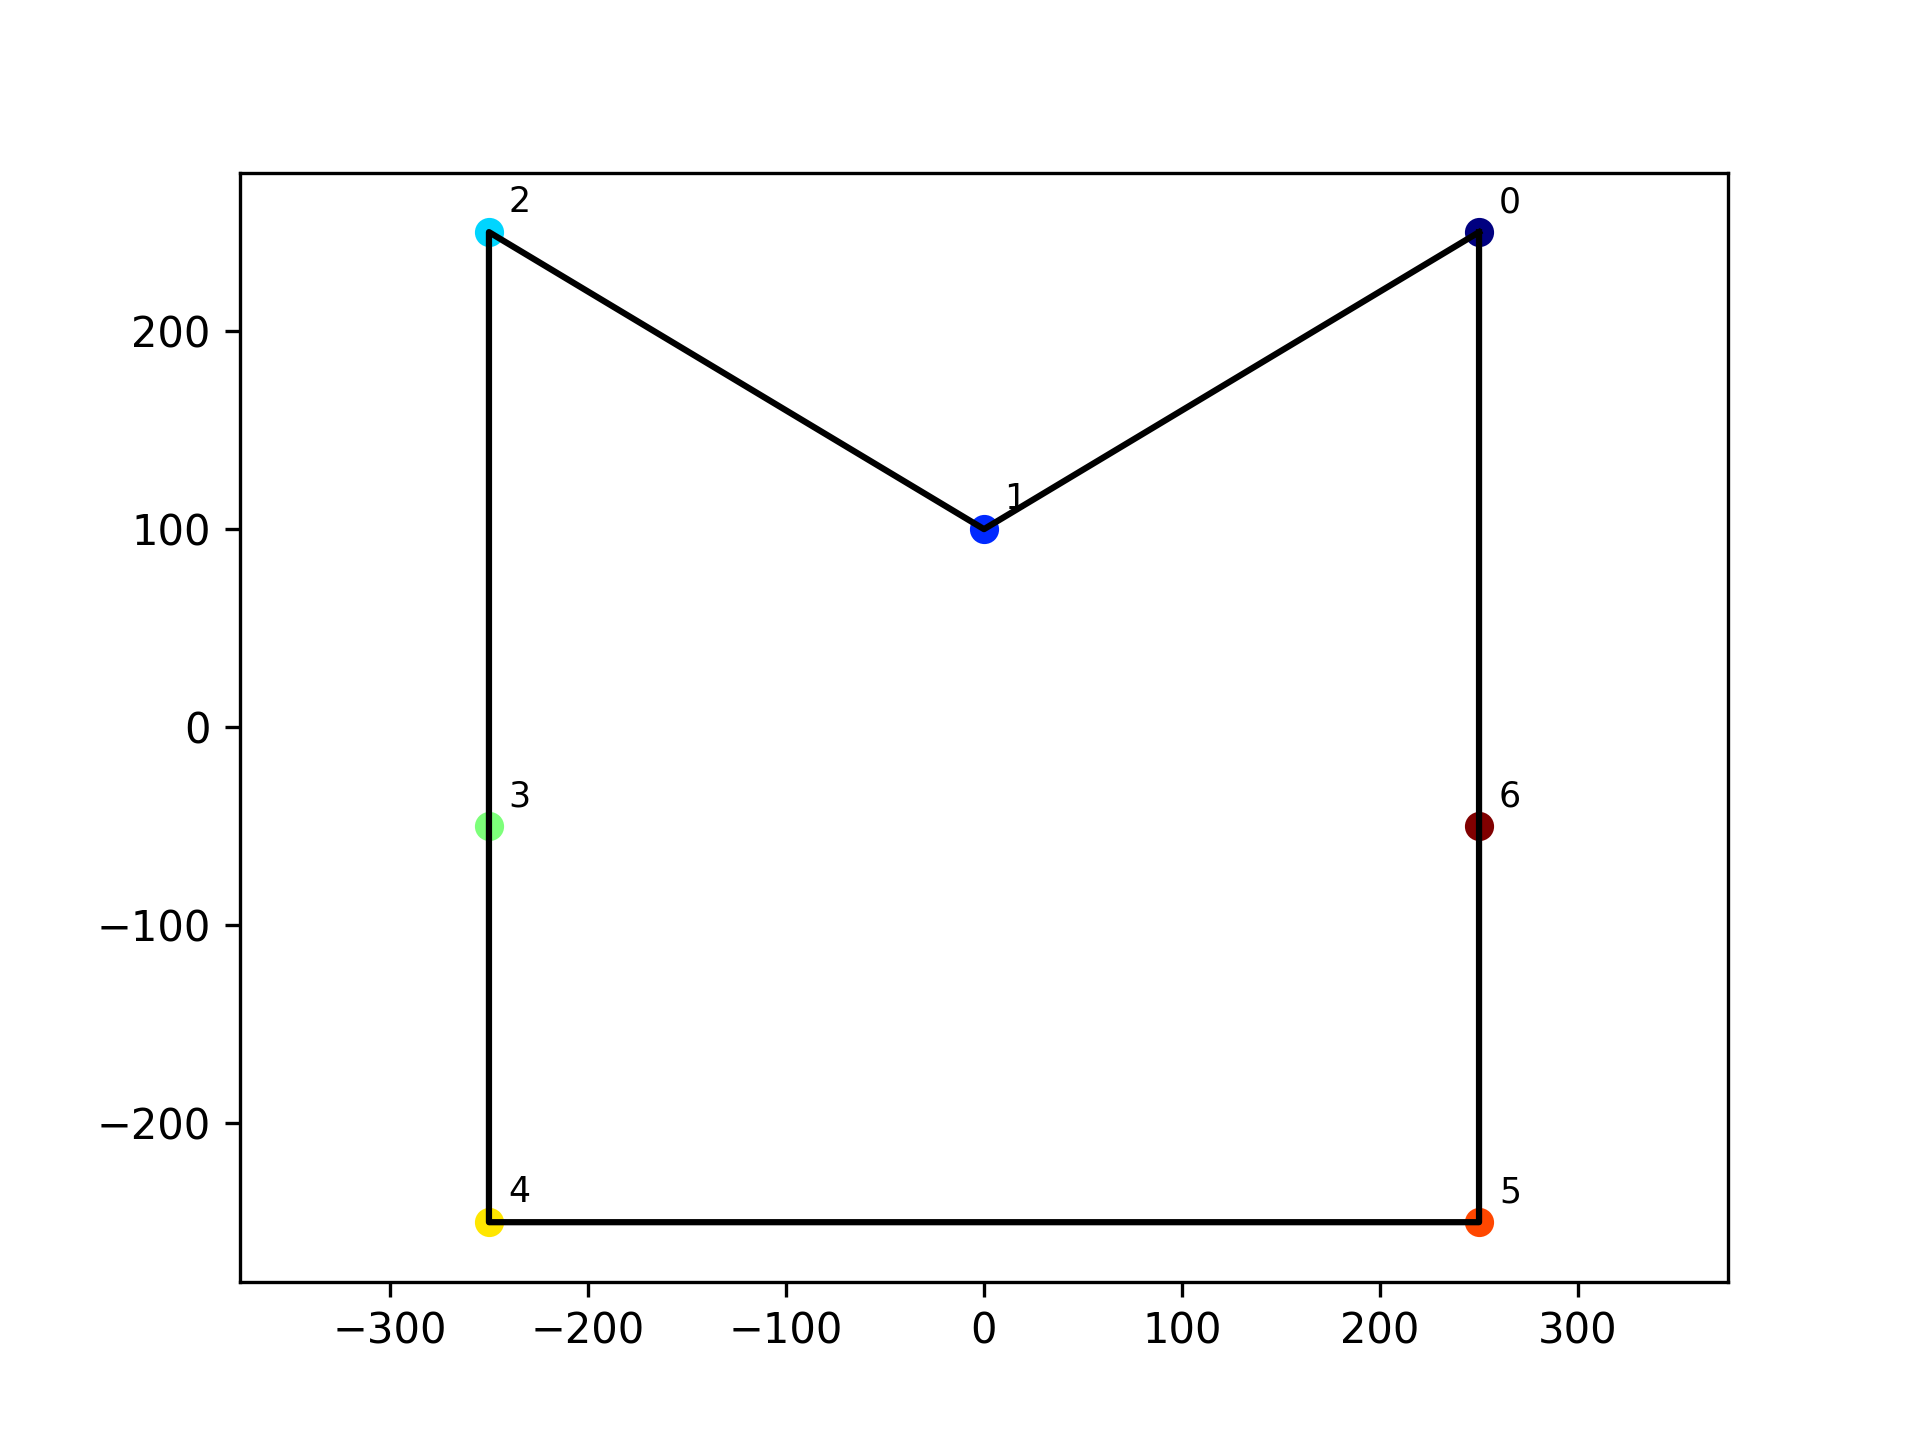
\includegraphics[width=\linewidth]{figures/simple_nonconv_augmented.png}
  \label{fig:sn1}
\end{subfigure}%
\begin{subfigure}{0.3\textwidth}
  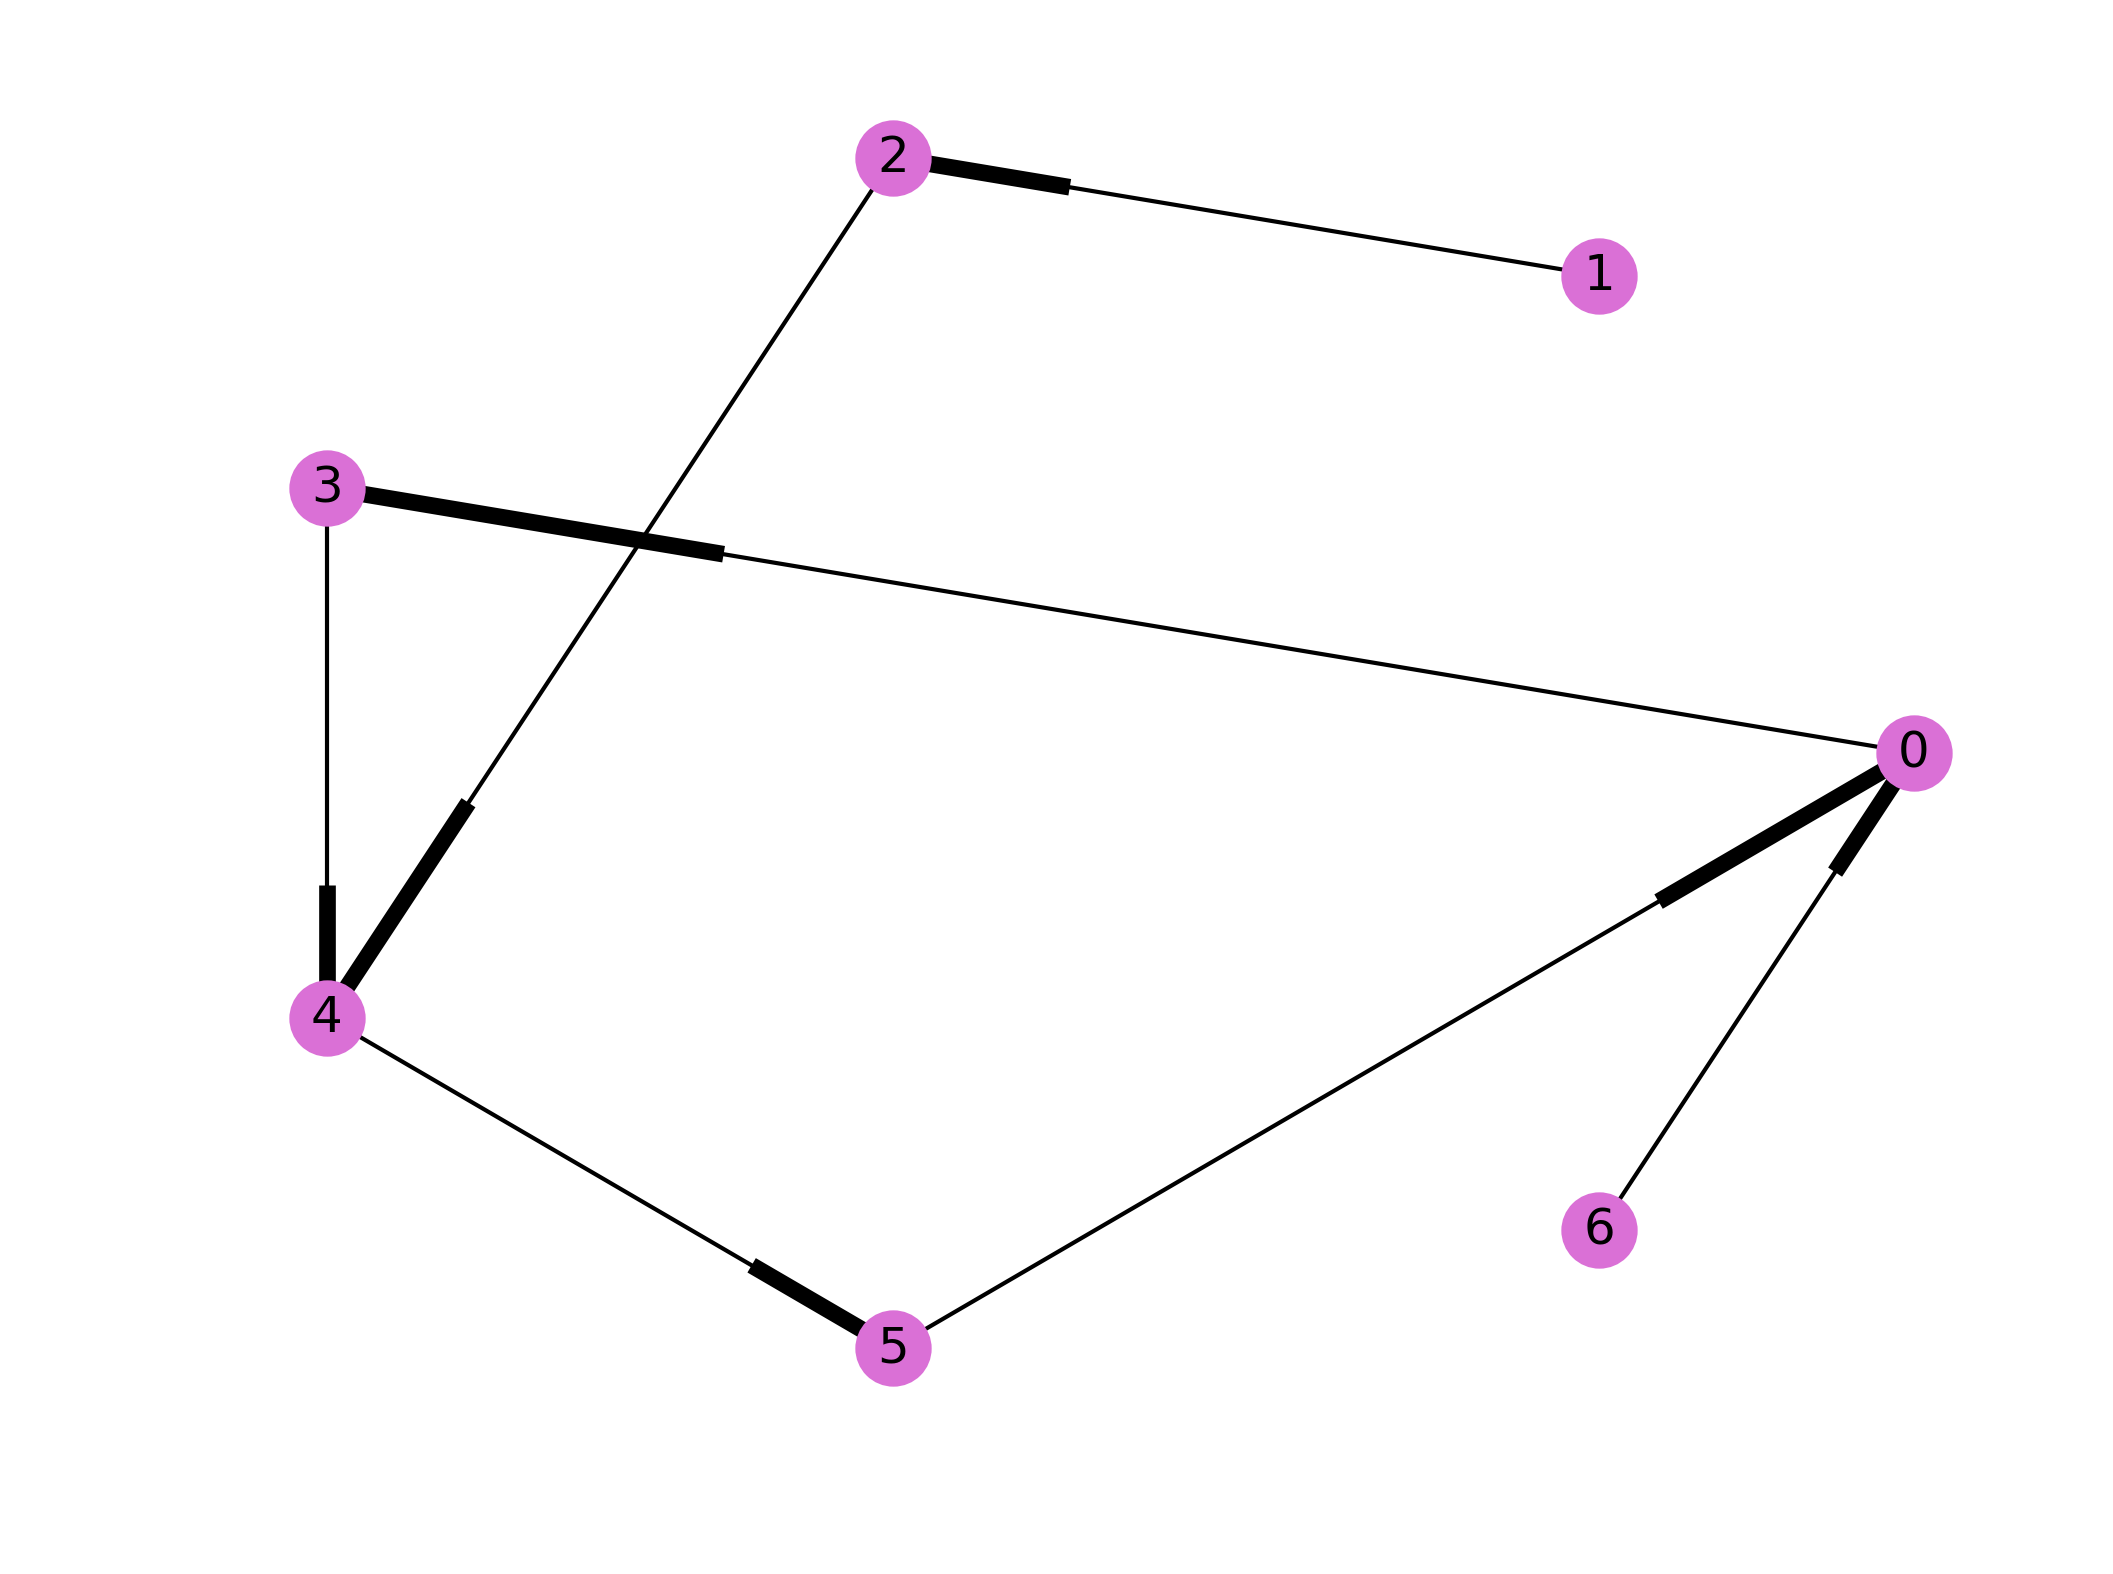
\includegraphics[width=\linewidth]{figures/simple_nonconv_BVD.png}
  \label{fig:sn2}
\end{subfigure}%
\begin{subfigure}{0.3\textwidth}
  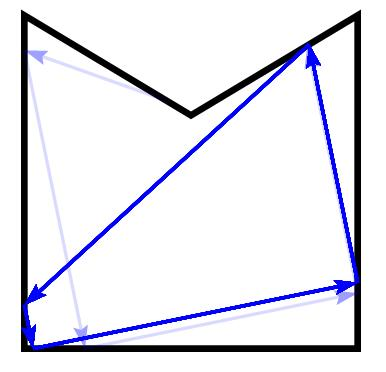
\includegraphics[width=\linewidth]{figures/simple_nonconv.jpg}
  \label{fig:sn3}
\end{subfigure}
\caption{\label{fig:sn}}

\end{figure}


\subsection{Localization}

We define the \emph{localization} task as:

\begin{quotation}
Given an accurate map of the environment, but no knowledge of configuration,
determine a strategy which eliminates uncertainty in configuration as much as
possible (ideally, to a point in configuration space).
\end{quotation}

In \cite{OkaLav06}, the authors show that localization is possible with
mobile robots with a linear and angular odometer, or a compass and contact
sensor, but not with robots with only an angular odometer and contact sensor.
These sensing configurations correspond to which types of bounce laws each robot
is capable of performing, and we would like to be able to rederive the same
results in this representation.

Localization amounts to a path finding algorithm in the larger graph, where each
node is an element of the powerset of segments along $P'$. Future work will
include how to tractibly search this graph (such as heuristics for doing so
which take advantage of the uncertainty-reducing properties of contraction
mappings).


\section{Open Questions and Future Work}

If a robot has some guaranteed minimum uncertainty in its actuation, we may
"trim" both ends of each angle interval in the strategy to determine if a "safe"
strategy exists under this actuation uncertainty.


Future work also includes:

\begin{itemize}
\item Characterizing the completeness and correctness of algorithms for
navigation, coverage, localization, etc.
\item Continue to place this work in context, especially with BitBots, Gap
Navigation Trees, and Combinatorial Visibility Vectors
\item Developing ways to query two $G_{BVD}$s, generated with different constraints on
 bouncing laws and sensors, and determine whether one represents a robot which
is ``more powerful" than another. Perhaps this will require a clever
parameterization of bouncing laws.
\item Investigate how to generate bounce law distributions that allow a bounce
to be randomly selected at each stage and guarantee some properties about the
resulting trajectory
\item Extending analysis to more tasks, such as coverage and pursuit-evasion
\end{itemize}


%\begin{tikzpicture}[->,>=stealth,auto,node distance=2.5cm,
%  thick,main node/.style={circle,draw,minimum size = 1.7cm, font=\scriptsize}]
%\node[main node] (x0)   [align=center] {$l_1$\\$x = 0$};
%\node[main node] (x01)  [align=center,below of=x0] {$l_1$\\$0 < x < 1$};
%\node[main node] (x1)   [align=center,below of=x01] {$l_1$\\$x = 1$};
%\node[main node] (x12)  [align=center,below of=x1] {$l_1$\\$1< x < 2$};
%\node[main node] (x2)   [align=center,below of=x12] {$l_1$\\$x = 2$};
%\node[main node] (x23)  [align=center,below of=x2] {$l_1$\\$2<x <3$};
%\node[main node] (x3)   [align=center,below of=x23] {$l_1$\\$x = 3$};
%\node[main node] (x34)  [align=center,below of=x3] {$l_1$\\$3< x < 4$};
%\node[main node] (x4)   [align=center,below of=x34] {$l_1$\\$x = 4$};
%
%\node[main node] (y0)   [align=center,right of=x0] {$l_2$\\$x = 0$};
%\node[main node] (y01)  [align=center,right of=x01] {$l_2$\\$0 < x < 1$};
%\node[main node] (y1)   [align=center,right of=x1] {$l_2$\\$x = 1$};
%\node[main node] (y12)  [align=center,right of=x12] {$l_2$\\$1< x < 2$};
%\node[main node] (y2)   [align=center,right of=x2] {$l_2$\\$x = 2$};
%\node[main node] (y23)  [align=center,right of=x23] {$l_2$\\$2<x <3$};
%\node[main node] (y3)   [align=center,right of=x3] {$l_2$\\$x = 3$};
%\node[main node] (y34)  [align=center,right of=x34] {$l_2$\\$3< x < 4$};
%\node[main node] (y4)   [align=center,right of=x4] {$l_2$\\$x = 4$};
%\node[main node] (y4p)  [align=center,right of=y4] {$l_2$\\$x > 4$};
%
%\path[every node/.style={font=\sffamily\small}]
%     (x0)   edge node [right] {} (x01)
%     (x01)  edge node [right] {} (x1)
%     (x1)   edge node [right] {} (x12)
%     (x12)  edge node [right] {} (x2)
%     (x2)   edge node [right] {} (x23)
%     (x23)  edge node [right] {} (x3)
%     (x3)   edge node [right] {} (x34)
%     (x34)  edge node [right] {} (x4)
%     
%     
%     
%     (y0)   edge node [right] {} (y01)
%     (y01)  edge node [right] {} (y1)
%     (y1)   edge node [right] {} (y12)
%     (y12)  edge node [right] {} (y2)
%     (y2)   edge node [right] {} (y23)
%     (y23)  edge node [right] {} (y3)
%     (y3)   edge node [right] {} (y34)
%     (y34)  edge node [right] {} (y4)
%     (y4)   edge node [right] {} (y4p)
%     (y4p)  edge [loop above] node {} (y4p) 
%     
%     (y1)   edge node [right] {} (x1)
%     (y12)  edge node [right] {} (x12)
%     (y2)   edge node [right] {} (x2)
%     (y23)  edge node [right] {} (x23)
%     (y3)   edge node [right] {} (x3)
%     (y34)  edge node [right] {} (x34)
%     (y4)   edge node [right] {} (x4);
%     
%    \draw [shorten >=1pt,->, smooth] plot coordinates {(x23.west) (-1, -10) (-1,1) (y0.north)};
%    \draw [shorten >=1pt,->, smooth] plot coordinates {(x3.west) (-1.5, -12) (-1.5, 1.5) 
%    (y0.north)};
%    \draw [shorten >=1pt,->, smooth] plot coordinates  {(x34.west) (-2, -14) (-2, 2)
%    (y0.north)};
%    \draw [shorten >=1pt,->, smooth] plot coordinates  {(x4.west) (-2.5, -16) (-2.5, 2.5)
%     (y0.north)};
%
%\end{tikzpicture}

\fi

\bibliographystyle{spmpsci}
\bibliography{refs}

\end{document}
